\documentclass{article}

\usepackage[utf8]{inputenc}
\usepackage{amsmath, amssymb, amsthm}
\usepackage[dvipsnames]{xcolor}
\usepackage{color}
\usepackage{tikz}
\usepackage{array}
\usepackage{pgfmath}
\usepackage{soul}
\usepackage{multirow}
\usepackage{colortbl}
\usepackage{pgfplots}
\usepackage{ulem}
\usepackage{extpfeil}
\usepackage[hidelinks]{hyperref}

\pgfplotsset{compat=1.18}
\usetikzlibrary{matrix}


\definecolor{dgr}{rgb}{0.72, 0.53, 0.04}
\definecolor{maroon}{rgb}{0.5, 0.0, 0.0}


\newcommand{\smsk}{\vspace{3px}}
\newcommand{\mesk}{\vspace{10px}}

\newcommand{\smsp}{\phantom{\hspace{3px}}}
\newcommand{\mesp}{\phantom{\hspace{10px}}}

\newcommand{\red}[1]{\textcolor{red}{#1}}
\newcommand{\gray}[1]{\textcolor{gray}{#1}}
\newcommand{\blue}[1]{\textcolor{blue}{#1}}
\newcommand{\green}[1]{\textcolor{green}{#1}}
\newcommand{\dgr}[1]{\textcolor{dgr}{#1}}
\newcommand{\maroon}[1]{\textcolor{maroon}{#1}}
\newcommand{\cyan}[1]{\textcolor{cyan}{#1}}

\newcommand{\hcyan}[1]{\colorbox{cyan}{#1}}
\newcommand{\hgreen}[1]{\colorbox{green}{#1}}

\newcommand{\ex}{\green{\textbf{Beispiel: }}}
\newcommand{\de}[1]{\red{\textbf{Definition: }}\begin{quote}#1\end{quote}}
\newcommand{\an}[1]{\blue{\textbf{Bemerkung: }}\begin{quote}#1\end{quote}}
\newcommand{\prop}[1]{\dgr{\textbf{Proposition: }}\begin{quote}#1\end{quote}}
\newcommand{\se}[1]{\dgr{\textbf{Satz: }}\begin{quote}#1\end{quote}}
\newcommand{\lem}[1]{\dgr{\textbf{Lemma: }}\begin{quote}#1\end{quote}}
\newcommand{\cl}[1]{\dgr{\textbf{Behauptung: }}\begin{quote}#1\end{quote}}
\newcommand{\co}[1]{\dgr{\textbf{Korollar: }}\begin{quote}#1\end{quote}}
\newcommand{\pr}[1]{\maroon{\textbf{Beweis: }}\begin{quote}#1\end{quote}\qed}

\newcommand{\n}[1]{\overline{#1}}
\newcommand{\N}{\mathbb{N}}
\newcommand{\Z}{\mathbb{Z}}
\newcommand{\Q}{\mathbb{Q}}
\newcommand{\R}{\mathbb{R}}
\newcommand{\C}{\mathbb{C}}
\newcommand{\vst}{\smsp \vline \smsp}
\renewcommand{\st}{\smsp | \smsp}

\newcommand{\xor}{\mathbin{\vartriangle}}
\newcommand{\no}[1]{||#1||}
\newcommand{\vvec}[2]{\begin{pmatrix}#1\\#2\end{pmatrix}}
\newcommand{\vvvec}[3]{\begin{pmatrix}#1\\#2\\#3\end{pmatrix}}
\newcommand{\vfec}[4]{\begin{pmatrix}#1\\#2\\#3\\#4\end{pmatrix}}

\renewcommand{\mod}{\text{ mod }}
\newcommand{\spann}[1]{\left\langle#1\right\rangle}
\newcommand{\col}{\text{col}}
\newcommand{\row}{\text{row}}
\newcommand{\rg}{\text{rg}}
\newcommand{\im}{\text{Im}}
\newcommand{\tr}{\text{Spur}}
\newcommand{\eig}{\text{Eig}}


\setlength{\parindent}{0pt}
\setlength{\parskip}{3pt} 


\title{Lineare Algebra}
\author{Daniel}
\date{October 2024}

\begin{document}

\maketitle
\tableofcontents

\newpage
\section{Der Körper der Komplexen Zahlen}

{\bf Komplexe Zahlen} haben viele Eigenschaften mit den reellen Zahlen gemeinsam besitzen darüber hinaus aber weitere Vorteilhafte Eigenschaften, die sich für die modernen Ingenieurwissenschaften als nützlich erwiesen haben.

In der Linearen Algebra werden komplexe Zahlen bei der Berechnung von Eigenwerten und Eigenvektoren von Matrizen benötigt (mit zahlreichen Anwendungen). In der Numerischen Mathematik werden die Eigenschaften komplexer Zahlen benötigt, um effizient mit sehr großen natürlichen Zahlen rechnen zu können.

Die komplexen Zahlen bilden als algebraische Struktur einen Körper. \\
In der gesamten Linearen Algebra werden ihre Eigenschaften für das Rechnen in Körpern ausgenutzt.

\phantomsection
\addcontentsline{toc}{subsection}{Einführung}
\subsubsection{Konstruktion der komplexen Zahlen}

Aus der Schule bekannte Zahlenbereiche:
\begin{equation*} \label{zahlenbereiche}
    \N \mesp \subseteq \mesp \Z \mesp \subseteq \mesp \Q \mesp \subseteq \mesp \R \mesp \red{\subseteq \mesp \C}
\end{equation*}
Wir konstruieren einen Zahlenbereich $\C$ mit folgenden Eigenschaften:
\begin{itemize}
    \item $\R \subseteq \C$
    \item $x^2 = -1$ ist in $\C$ lösbar
    \item Es gelten die Rechengesetze aus $\R$
    \item $\C$ ist so klein wie möglich
\end{itemize}
\de{\red{$i$} mit $i^2 = -1$ heißt \red{imaginäre Einheit}}

\begin{table}[ht]
    \centering
    \begin{tabular}{m{5cm} m{5cm}}
        \an{\begin{itemize}
            \item $i \subseteq \C$
            \item $a, b  \in \R$
        \end{itemize}} &
        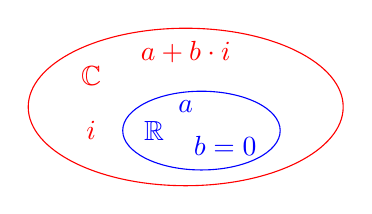
\begin{tikzpicture}
            \draw[draw=red] (0,0) ellipse(2cm and 1cm);
            \node at (-1.2, 0.4) {{\color{red}$\C$}};
            \node at (0, 0.7) {{\color{red}$a + b \cdot i$}};
            \node at (-1.2, -0.3) {{\color{red}$i$}};
    
            \draw[draw=blue] (0.2,-0.3) ellipse(1cm and 0.5cm);
            \node at (-0.4, -0.3) {{\color{blue}$\R$}};
            \node at (0, 0) {{\color{blue}$a$}};
            \node at (0.5, -0.5) {{\color{blue}$b = 0$}};
        \end{tikzpicture}
    \end{tabular}
\end{table}

\de{
    $\red{\C := \{a + b \cdot i \mid a, b \in \R\}}$ ist die Menge der komplexen Zahlen. Für $z = a + b \cdot i \in \C$ heißt $Re(z) := a$ der Realteil von $z$ und $Im(z) := b$ heißt der Imaginärteil von $z$
}

\subsection{Komplexe Zahlen in arithmetischer Schreibweise}
\subsubsection{Rechenregeln}

Der Körper der komplexen Zahlen ist ($\C; +, *$).\\
Die komplexen Zahlen haben folgende Eigenschaften:
\begin{itemize}
    \item $+$ ist assoziativ:
        \begin{equation*}
            (z_1 + z_2) + z_3 = z_1 + (z_2 + z_3) \mesp \text{für alle } z_1, z_2, z_3 \in \C
        \end{equation*}
    \item $+$ ist kommutativ:
        \begin{equation*}
            z_1 + z_2 = z_2 + z_1 \mesp \text{für alle } z_1, z_2 \in \C
        \end{equation*}
    \item $+$ hat ein neutrales Element 0:
        \begin{equation*}
            z + 0 = 0 + z = z \mesp \text{für alle } z \in \C 
        \end{equation*}
    \item Jedes Element $z \in \C$ hat ein Inverses -z bezüglich $+$:
        \begin{equation*}
            z + (-z) = (-z) + z = 0
        \end{equation*}
    \item $*$ ist assoziativ:
        \begin{equation*}
            (z_1 \cdot z_2) \cdot z_3 = z_1 \cdot (z_2 \cdot z_3) \mesp \text{für alle } z_1, z_2, z_3 \in \C
        \end{equation*}
    \item $*$ ist kommutativ:
        \begin{equation*}
            z_1 \cdot z_2 = z_2 \cdot z_1 \mesp \text{für alle } z_1, z_2 \in \C
        \end{equation*}
    \item $+$ hat ein neutrales Element 1:
        \begin{equation*}
            z \cdot 1 = 1 \cdot z = z \mesp \text{für alle } z \in \C 
        \end{equation*}
    \item Jedes Element $z \in \C \backslash \{0\}$ hat ein Inverses $z^{-1}$ bezüglich $*$:
        \begin{equation*}
            z \cdot z^{-1} = z^{-1} \cdot z = 1
        \end{equation*}
    \item $*$ ist distributiv bezüglich $+$:
        \begin{equation*}
            z_1 \cdot (z_2 + z_3) = z_1 \cdot z_2 + z_1 \cdot z_3 \mesp \text{für alle } z_1, z_2, z_3 \in \C
        \end{equation*}
\end{itemize}

\newpage
\subsubsection{Rechnen mit komplexen Zahlen}

$\C = \{a + bi \mid a, b\}$ ist die Menge der komplexen Zahlen

\begin{itemize}
    \item Addieren:
        \begin{equation*}
            (a + bi) + (c + di) := (a + c) + (b + d)i
        \end{equation*}
    \item Subtrahieren
        \begin{equation*}
            (a + bi) - (c + di) := (a - c) + (b - d)i
        \end{equation*}
    \item Multiplizieren
        \begin{equation*}
            (a + bi) \cdot (c + di) := (ac - bd) + (ad + bc)i
        \end{equation*}
    \item Dividieren
        \begin{equation*}
            \frac{a + bi}{c + di} := \frac{ac + bd}{c^2 + d^2} + \frac{bc - ad}{c^2 + d^2}i \mesp \text{für } c + di \neq 0
        \end{equation*}
\end{itemize}

Um komplexe Zahlen in arithmetischer Form einfacher zu dividieren wird ein "Standardtrick" verwendet:
\begin{equation*}
    \begin{array}{lcl}
        (1 + 2i) : (3 - 4i) & = & \frac{(1 + 2i)}{(3 - 4i)} \\[10pt]
                            & = & \frac{(1 + 2i)}{(3 - 4i)} \cdot {\color{red} 1} \\[10pt]
                            & = & \frac{(1 + 2i)}{(3 - 4i)} \cdot {\color{red} \frac{3 + 4i}{3 + 4i}} \\[10pt]
                            & = & \frac{(1 + 2i) \cdot (3 + 4i)}{(3 - 4i) \cdot (3 + 4i)} \\[10pt]
                            & = & \frac{-5 + 10i}{25} \\[10pt]
                            & = & -\frac{1}{5} + \frac{2}{5}i
    \end{array}
\end{equation*}

\subsection{Konjugiert komplexe Zahlen}

\de{Sei $z := a + bi \in \C$. Dann nennt man $\bar{z} := a - bi$ die zu z konjugiert komplexe Zahl.}
\an{Man dividiert durch eine komplexe Zahl $z \neq 0$, indem man mit der konjugiert komplexen Zahl erweitert.}

\an{Sei $a + bi \in \C \backslash {0}$, dann gilt:}
\begin{equation*}
    (a + bi)^{-1} = \frac{1}{a + bi} = \frac{1}{a + bi} \cdot {\color{red}\frac{a - bi}{a - bi}} = \frac{a - bi}{a^2 + b^2} = \frac{a}{a^2 + b^2} - \frac{b}{a^2 + b^2}i
\end{equation*}

\subsection{\texorpdfstring{GAUSS'sche Zahlenebene, kartesische Koordinaten, \\Polarkoordinaten}{GAUSS'sche Zahlenebene, kartesische Koordinaten, Polarkoordinaten}}

\an{Komplexe Zahlen $z$ kann man in der Form $z = a + bi \mesp (a, b \in \R)$
darstellen. Diese Darstellung nennt man {\bf arithmetische\\Darstellung} von $z$. Komplexe Zahlen kann man in arithmetischer Darstellung leicht addieren, sowie subtrahieren und aufwendiger multiplizieren, sowie dividieren.

Um komplexe Zahlen leicht multiplizieren und dividieren zu können werden noch die trigonometrische Darstellung und die EULERsche Darstellung Komplexer Zahlen eingeführt.}


\begin{table}[h!]
    \centering
    \begin{tabular}{m{6.5cm} m{4.7cm}}
        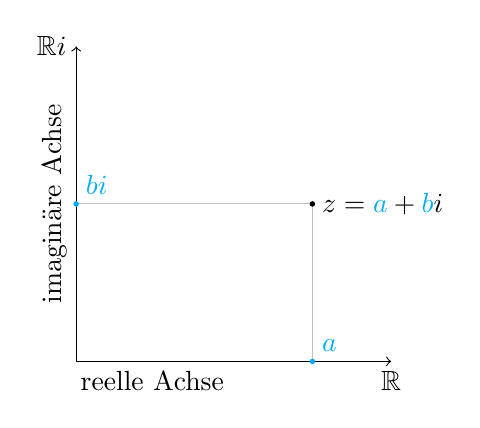
\begin{tikzpicture}
            \draw[black, ->] (0,0) -- (0,4) node[above, left] {$\R i$};
            \node[rotate=90, above] at (0,2) {imaginäre Achse};
            \draw[black, ->] (0,0) -- (4,0) node[below] {$\R$};
            \node[below left] at (2,0) {reelle Achse};
            \draw[lightgray] (3,0) -- (3,2);
            \draw[lightgray] (0,2) -- (3,2);
            \fill[cyan] (3,0) circle (1pt) node[above right] {$\cyan{a}$};
            \fill[cyan] (0,2) circle (1pt) node[above right] {${\cyan{b}}{i}$};
            \fill[black] (3,2) circle (1pt) node[right] {$z = {\cyan{a}} + {\cyan{b}}i$};
        \end{tikzpicture}&
        $z = \cyan{a} + \cyan{b}i$ hat die

        \cyan{\fcolorbox{cyan}{white} {\parbox{4cm}{kartesischen Koordinaten\\\centering (a, b)}}}\smsk

        \cyan{$a$} ist der Realteil von  $z$

        \cyan{$b$} ist der Imaginärteil von  $z$
        \\
        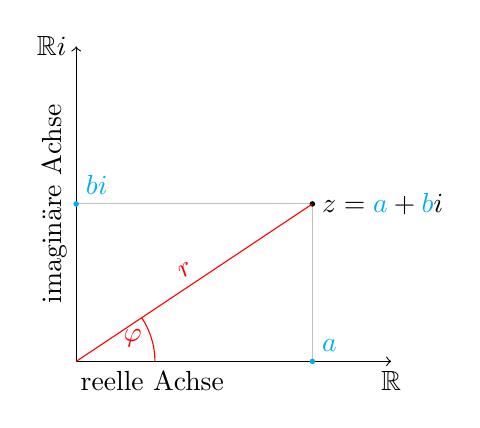
\begin{tikzpicture}
            \draw[black, ->] (0,0) -- (0,4) node[above, left] {$\R i$};
            \node[rotate=90, above] at (0,2) {imaginäre Achse};
            \draw[black, ->] (0,0) -- (4,0) node[below] {$\R$};
            \node[below left] at (2,0) {reelle Achse};
            \draw[lightgray] (3,0) -- (3,2);
            \draw[lightgray] (0,2) -- (3,2);
            \fill[cyan] (3,0) circle (1pt) node[above right] {$\cyan{a}$};
            \fill[cyan] (0,2) circle (1pt) node[above right] {${\cyan{b}}{i}$};
            \fill[black] (3,2) circle (1pt) node[right] {$z = {\cyan{a}} + {\cyan{b}}i$};
            \draw[red] (0,0) -- (3,2) node[midway, above, rotate=33.7] {$r$};
            \draw[red] (1,0) arc[start angle=0, end angle=33.7, radius=1] node[midway, left] {$\varphi$};
        \end{tikzpicture} &
        $z = \cyan{a} + \cyan{b}i$ hat die\smsk

        {\color{red} \fcolorbox{red}{white} {\parbox{4cm}{Polarkoordinaten\\\centering ($r$, $\varphi$)}}}
    \end{tabular}
\end{table}

\red{$r$} ist der Betrag von $z$: $|z| := r = \sqrt{a^2 + b^2}$

\red{$\varphi$} ist das Argument von $z$: $Arg(z) := \varphi \mesp$mit
\begin{tabular}{l}
    $\sin(\varphi) = \frac{b}{r}$, \\
    $\cos(\varphi) =  \frac{a}{r}$
\end{tabular}
\smsk

Umrechnung \mesp
\cyan{\fcolorbox{cyan}{white} {\parbox{4cm}{kartesischen Koordinaten\\\centering (a, b)}}} 
$\longleftrightarrow$
\red{\fcolorbox{red}{white} {\parbox{4cm}{Polarkoordinaten\\\centering ($r$, $\varphi$)}}}

\begin{itemize}
    \item 
    \begin{tabular}{l l}
        $\red{(r, \varphi)} \rightarrow \cyan{(a, b)}$: & 
        \begin{tabular}{l}
            ${\color{cyan}a} = {\color{red}r} \cdot \cos(\red{\varphi})$\\
            ${\color{cyan}b} = {\color{red}r} \cdot \sin(\red{\varphi})$
        \end{tabular}
    \end{tabular}
    \item 
    \begin{tabular}{l l}
        ${\cyan{(a, b)}} \rightarrow {\red{(r, \varphi)}}$: & 
        \begin{tabular}{l}
            ${\red{r}} = \sqrt{\cyan{a}^2 + \cyan{b}^2}$\\
            Durch $\sin(\red{\varphi}) = \frac{\red{b}}{\red{r}}$ UND $\cos(\red{\varphi}) = \frac{\cyan{a}}{\red{r}}$ ist $\red{\varphi \in[0, 2 \pi)}$\\
            eindeutig bestimmt.
        \end{tabular}
    \end{tabular}\\
    Es genügt nicht, zur Bestimmung von $\varphi$ nur eine dieser beiden Gleichungen zu betrachten.
\end{itemize}

\underline{Darstellung komplexer Zahlen $z  \in \C$}

\begin{itemize}
    \item 
    \begin{tabular}{l r}
        \begin{tabular}{l}
            arithmetische Darstellung:\\
            \cyan{(kartesische Koordinaten)}
        \end{tabular}
        \hspace{24px}
        \begin{tabular}{r}
            \large\fcolorbox{cyan}{white} {$z = a + bi$}
        \end{tabular}    
    \end{tabular}
    \item 
    \begin{tabular}{l r}
        \begin{tabular}{l}
            trigonometrische Darstellung:\\
            \red{(Polarkoordinaten)}
        \end{tabular}
        \hspace{10px}
        \begin{tabular}{r}
            \large\fcolorbox{red}{white} {$z = r (\cos(\varphi) + i \cdot \sin(\varphi))$}
        \end{tabular}    
    \end{tabular}
    \item 
    \begin{tabular}{l r}
        \begin{tabular}{l}
            EULERsche Darstellung:\\
            \red{(Polarkoordinaten)}
        \end{tabular}
        \hspace{30px}
        \begin{tabular}{r}
            \large\fcolorbox{red}{white} {$z = r \cdot e^{i \cdot \varphi}$}
        \end{tabular}    
    \end{tabular}
\end{itemize}

\subsection{\texorpdfstring{Rechnen mit komplexen Zahlen \\in EULERscher Darstellung}{Rechnen mit komplexen Zahlen in EULERscher Darstellung}}

Sei $z_1 = r_1 \cdot e^{i\varphi_1}$, $z_2 = r_2 \cdot e^{i\varphi_2}$
\begin{itemize}
    \item Multiplikation: $z_1 \cdot z_2 = r_1 \cdot e^{i\varphi_1} \cdot r_2 \cdot e^{i\varphi_2} = r_1r_2 \cdot e^{i\varphi_1 + i\varphi_2}$
    \begin{equation*}
        \hspace{-50px} \implies \hspace{10px} \fcolorbox{black}{white} {$r_1r_2 \cdot e^{i(\varphi_1 + \varphi_2)}$}
    \end{equation*}
    \item Division: $z_1 : z_2 = \frac{z_1}{z_2} = \frac{r_1 \cdot e^{i\varphi_1}}{r_2 \cdot e^{i\varphi_2}} = \frac{r_1}{r_2} \cdot e^{i\varphi_1 - i\varphi_2}$
    \begin{equation*}
        \hspace{-50px} \implies \hspace{10px} \fcolorbox{black}{white} {$\frac{r_1}{r_2} \cdot e^{i(\varphi_1 - \varphi_2)}$}
    \end{equation*}
\end{itemize}

\newpage

\section{\texorpdfstring{Lineare Gleichungssysteme und Matrizen \\über einen Körper K}{Lineare Gleichungssysteme und Matrizen über einen Körper K}}

Betrachtet werden in diesem Kapitel ausschließlich die folgenden Körper:
\begin{itemize}
    \item Körper der reellen Zahlen $(\R; +, \cdot)$
    \item Körper der komplexen Zahlen $(\C; +, \cdot)$
    \item endlicher Körper $(GF(2); +, \cdot)$ mit $GF(2) = \{0, 1\}$ und
    
    \begin{tabular}{m{2cm} m{3.5cm} m{3.5cm}}
        Galois-Field&
        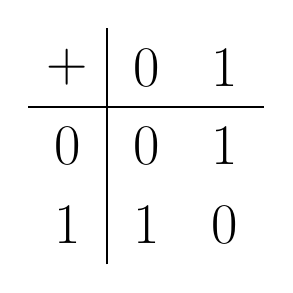
\begin{tikzpicture}
            \draw[black] (1,0) -- (1,3);
            \draw[black] (0, 2) -- (3,2);
            \node[] at (0.5,2.5) {\huge$+$};
            \node[] at (0.5,1.5) {\huge$0$};
            \node[] at (0.5,0.5) {\huge$1$};
            \node[] at (1.5,2.5) {\huge$0$};
            \node[] at (2.5,2.5) {\huge$1$};
            \node[] at (1.5,1.5) {\huge$0$};
            \node[] at (1.5,0.5) {\huge$1$};
            \node[] at (2.5,0.5) {\huge$0$};
            \node[] at (2.5,1.5) {\huge$1$};
        \end{tikzpicture} &
        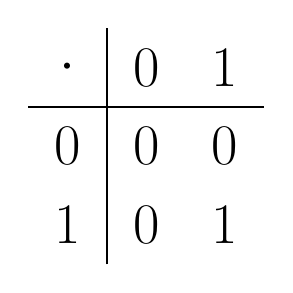
\begin{tikzpicture}
            \draw[black] (1,0) -- (1,3);
            \draw[black] (0, 2) -- (3,2);
            \node[] at (0.5,2.5) {\huge$\cdot$};
            \node[] at (0.5,1.5) {\huge$0$};
            \node[] at (0.5,0.5) {\huge$1$};
            \node[] at (1.5,2.5) {\huge$0$};
            \node[] at (2.5,2.5) {\huge$1$};
            \node[] at (1.5,1.5) {\huge$0$};
            \node[] at (1.5,0.5) {\huge$0$};
            \node[] at (2.5,0.5) {\huge$1$};
            \node[] at (2.5,1.5) {\huge$0$};
        \end{tikzpicture}
    \end{tabular}
\end{itemize}

\subsection{Lineare Gleichungen und lineare Gleichungssysteme}

\de{Sei K ein Körper, so heißt $a_1 \cdot x_1 + a_2 \cdot x_2 + \dots + a_n \cdot x_n = b$ (mit $n \in \N)$ eine \red{lineare Gleichung} in den Unbekannten $x_1, x_2, \dots, x_n$ über K.

Kurz:
\begin{equation*}
    \sum_{j = 1}^{n} a_j \cdot x_j = b
\end{equation*}} 
\gray{$b$ wir als Absolutglied bezeichnet}

\de{Sei K ein körper, so heißt $a_{i1} \cdot x_1 + a_{i2} \cdot x_2 + \dots + a_{in} \cdot x_n = b_i$ (mit $n \in \N$ und $i = 1, 2, 3, \dots, m$) \red{Lineares Gleichungssystem (LGS)} in den Unbekannten $x_1, x_2, \dots, x_n$ über K.

Kurz: 
\begin{equation*}
    \sum_{j = 1}^{n} a_{ij} \cdot x_j = b_i
\end{equation*}}
\gray{Ein LGS ist also die Zusammenfassung \red{m}ehrerer linearer Gleichungen}

\newpage
\subsubsection{Lösung eines linearen Gleichungssystems}

\de{Das n-Tupel $(l_1, l_2, \dots, l_n)$ mit $l_1, l_2, \dots, l_n \in K$ heißt \red{Lösung} des LGS, wenn sich beim Einsetzen eine wahre Aussage ergibt, d.h. wenn gilt:
\begin{equation*}
    \sum_{j = 1}^{n} a_{ij} \cdot l_j = b_i \smsp (\text{mit } i = 1, 2, \dots, m)
\end{equation*} 
Die Menge L aller Lösungen des LGS heißt \red{Lösungsmenge} des LGS.}

Es gibt zwei Arten linearer Gleichungssysteme:
\begin{itemize}
    \item homogenes LGS: 
    \begin{equation*}
        \sum_{j = 1}^{n} a_{ij} \cdot x_j = 0 \smsp (\text{mit } i = 1, 2, \dots, m)
    \end{equation*}
    \an{Ein homogenes LGS hat immer eine Lösung $(\red{0}, \red{0}, \dots, \red{0})$}
    \pr{$\sum_{j = 1}^{n} a_{ij} \cdot \red{0} = 0$ mit ($i = 1, 2, \dots, m$) ist eine wahre Aussage}
    \item inhomogenes LGS:
    \begin{equation*}
        \sum_{j = 1}^{n} a_{ij} \cdot x_j = b_i \smsp (\text{mit } i = 1, 2, \dots, m)
    \end{equation*}
    wobei (mindestens) ein $b_i \neq 0$

    \an{Ein inhomogenes LSG hat nicht die Lösung $(0, 0, \dots, 0)$}
\end{itemize}

\subsection{Matrizen}

\de{Sei $m, n \in \N \backslash \{0\}$, so ist die $m \times n$ - Matrix $A$ über dem Körper $K$ eine Abbildung
\begin{equation*}
    A: \{1, 2, \dots, m\} \times \{1, 2, \dots, n\} \rightarrow K: (i, j) \mapsto a_{ij}
\end{equation*}}

\newpage

\an{Matrizen sind spezielle Abbildungen (Funktionen). $m \times n$-Matrizen lassen sich als rechteckiges Schema mit $m$ Zeilen und $n$ Spalten notieren:}
\begin{equation*}
    A = 
    \begin{pmatrix}
        a_{11} & a_{12} & \dots & a_{1n} \\
        a_{21} & a_{22} & \dots & a_{2n} \\
        \vdots & \vdots & \ddots & \vdots \\
        a_{m1} & a_{m2} & \dots & a_{mn}
    \end{pmatrix}
    = (a_{ij})_{
       \begin{tabular}{c}
            \small $i = 1, 2, \dots, m$ \\
            \small $j = 1, 2, \dots, n$
            
        \end{tabular}
    }
    = (a_{ij})_{m \times n}
\end{equation*}

\an{$K^{m \times n}$ ist die Menge aller $m \times n$-Matrizen über $K$}

\subsubsection{Spezielle Matrizen}
\begin{itemize}
    \item Eine $m \times n$-Matrix heißt \red{quadratisch}, wenn $m = n$ gilt. Eine quadratische Matrix $A \in K^{n \times n}$ wird auch $n$-reihige Matrix genannt.
    \begin{equation*}
        A = 
    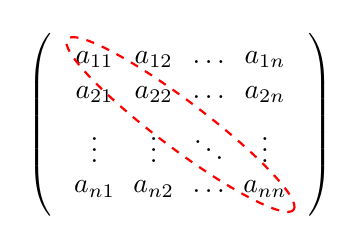
\begin{tikzpicture}[baseline={(current bounding box.center)}]
        \matrix (m) [matrix of math nodes,left delimiter={(},right delimiter={)}]{
            a_{11} & a_{12} & \dots & a_{1n} \\
            a_{21} & a_{22} & \dots & a_{2n} \\
            \vdots & \vdots & \ddots & \vdots \\
            a_{n1} & a_{n2} & \dots & a_{nn} \\
        };
        \draw[red, thick, dashed, rotate={-37}] ellipse (1.8cm and 0.3cm);
    \end{tikzpicture}
    \end{equation*}
    \gray{Bei der \red{Hauptdiagonale} gilt $i = j$}
    \item \red{Diagonalmatrix}: $D = (a_{ij})_{n \times n}$ mit $a_{ij} = 0$ für $i \neq j$\\
    \gray{Bis auf die Hauptdiagonale sind alle Werte in der Matrix $0$}
    \item \red{Einheitsmatrix}: $E = (a_{ij})_{n \times n}$ mit $a_{ij} =$
    $\begin{cases}
        1 & \text{für } i = j \\
        0 & \text{für } i \neq j
    \end{cases}$

    \gray{Diagonalmatrix, wobei alle Werte in der Hauptdiagonalen $1$ sind}
    \item \red{Nullmatrix}: $\mathbf{0}_{m \times n} = (a_{ij})_{m \times n}$ mit $a_{ij} = 0$ für all $i, j$\\
    \gray{Alle Werte in der Matrix sind $0$}
\end{itemize}

\newpage

\subsubsection{Rechnen mit Matrizen}

\begin{itemize}
    \item Addition: Sei $A = (a_{ij})_{m \times n}$, $B = (b_{ij})_{m \times n}$. Dann gilt:
    \begin{equation*}
        A + B := (a_{ij} + b_{ij})_{m \times n}
    \end{equation*}
    \an{Matrizen können nur addiert werden, wenn ihre Dimensionen übereinstimmen.}
    \ex
    \begin{equation*}
        A = \begin{pmatrix}
            1 & 2 & 3 \\
            4 & 5 & 6
        \end{pmatrix},
        B = \begin{pmatrix}
            2 & 1 & 0 \\
            0 & -1 & -3
        \end{pmatrix}
        \implies
        A + B = \begin{pmatrix}
            3 & 3 & 3\\
            4 & 4 & 3
        \end{pmatrix}
    \end{equation*}

    \item Multiplikation: Sei $A = (a_{ij})_{\cyan{m} \times \green{p}}$, $B = (a_{ij})_{\green{p} \times \red{n}}$. Dann gilt:
    \begin{equation*}
        A \cdot B := C \text{ mit } C = (c_{ij})_{\cyan{m} \times \red{n}} \text{ und } c_{ij} = \sum_{k = 1}^{\green{p}} a_{ik} \cdot b_{kj}
    \end{equation*}
    \an{Eine Matrix $A$ kann mit einer Matrix $B$ multipliziert werden, wenn die Spaltenanzahl der Matrix $A$ mit der Zeilenanzahl der Matrix $B$ übereinstimmt.}
    \gray{Diese Definition der Multiplikation von Matrizen modelliert die Hintereinanderausführung von linearen Abbildungen von Verkorräumen}

    \an{Zur Berechnung von $c_{ij}$ benötigt man nur die $i$-te Zeile von $A$ und die $j$-te Spalte von $B$:}
    \begin{equation*}
        a_{i1} \cdot b_{1j} + a_{i2} \cdot b_{2j} + \dots + a_{ip} \cdot b_{pj} = c_{ij}
    \end{equation*}
    \ex
    $A = \begin{pmatrix}
        1 & 2\\
        4 & 5\\
        7 & 8\\
    \end{pmatrix}$,
    $B = \begin{pmatrix}
        10 & 12\\
        11 & 14
    \end{pmatrix}$

    $A \cdot B$ ist eine Matrix mit 3 Zeilen und zwei Spalten:

    \begin{equation*}
        A \cdot B = \begin{pmatrix}
            1 \cdot 10 + 2 \cdot 11 & 1 \cdot 12 + 2 \cdot 14\\
            4 \cdot 10 + 5 \cdot 11 & 4 \cdot 12 + 5 \cdot 14\\
            7 \cdot 10 + 8 \cdot 11 & 7 \cdot 12 + 8 \cdot 14
        \end{pmatrix}
        = \begin{pmatrix}
            32 & 40\\
            95 & 118\\
            158 & 196
        \end{pmatrix}
    \end{equation*}
    $B \cdot A$ existiert nicht, da die Spaltenanzahl von $B$ nicht mit der Zeilenanzahl von $A$ übereinstimmt.

    \newpage

    \item Skalarmultiplikation: Sei $A = (a_{ij})_{m \times n}$, $k \text{ \gray{(Skalar)}} \in K$, dann gilt:
    \begin{equation*}
        k \cdot A := (k \cdot a_{ij})_{m \times n} = \begin{pmatrix}
            k \cdot a_{11} & k \cdot a_{12} & \dots & k \cdot a_{1n}\\
            k \cdot a_{21} & k \cdot a_{22} & \dots & k \cdot a_{2n}\\
            \vdots & \vdots & \ddots & \vdots\\
            k \cdot a_{m1} & k \cdot a_{m2} & \dots & k \cdot a_{mn}
        \end{pmatrix}     
    \end{equation*}
    \an{Eine Matrix wird mit einem Skalar multipliziert, indem man jedes Matrixelement mit diesem Skalar multipliziert}
    \ex \begin{equation*}
        5 \cdot \begin{pmatrix}
            1 & 2\\
            0 & 3\\
            -1 & 4
        \end{pmatrix}
        = \begin{pmatrix}
            5 & 10\\
            0 & 15\\
            -5 & 20
        \end{pmatrix}
    \end{equation*}

    \item Transponieren einer Matrix: Sei $A = (a_{ij})_{\cyan{m} \times \red{n}}$, dann gilt:
    \begin{equation*}
        A^T := (b_{ij})_{\red{n} \times \cyan{m}} \text{ mit } b_{ij} = a_{ji} 
    \end{equation*}
    $A^T$ heißt die \red{zu $A$ transponierte Matrix}\\
    \ex \begin{equation*}
        A = \begin{pmatrix}
            \red{1} & \cyan{2}\\
            \red{3} & \cyan{4}\\
            \red{5} & \cyan{6}
        \end{pmatrix}
        \implies
        A^T = 
        \begin{pmatrix}
            \red{1} & \red{3} & \red{5}\\
            \cyan{2} & \cyan{4} & \cyan{6}
        \end{pmatrix}
    \end{equation*}
\end{itemize}

\subsubsection{Rechenoperationen für Matrizen}

\begin{itemize}
    \item Addition (für alle $A, B, C \in K^{m \times n}$)
    \begin{itemize}
        \item $A + B = B + A$ (Kommutativgesetz)
        \item $(A + B) + C = A + (B + C)$ (Assoziativgesetz)
        \item $A + \mathbf{0} = A$ (Neutrales Element)
    \end{itemize}
    \item Multiplikation
    \begin{itemize}
        \item $(A \cdot B) \cdot C = A \cdot (B \cdot C)$ (Assoziativgesetz) (falls die Produkte $A \cdot B$ und $B \cdot C$ definiert sind)
        \item Es gilt $A \cdot E_n = E_n \cdot A = A$ für alle $A \in K^{n \times n}$\\
        \gray{$E_n$ ist die Einheitsmatrix mit $n$ Zeilen und $n$ Spalten}
        \item Es gilt $A \cdot \mathbf{0}_{m \times n} = \mathbf{0}_{m \times n}$ für alle $A \in K^{m \times n}$
    \end{itemize}

    \newpage

    \item Distributivgesetz (falls die entsprechenden Summen und Produkte existieren)
    \begin{itemize}
        \item $A \cdot (B + C) = (A \cdot B) + (A \cdot C)$
        \item $(B + C) \cdot A = (B \cdot A) + (C \cdot A)$
    \end{itemize}
    \item Transponieren (falls die entsprechenden Summen und Produkte von Matrizen existieren)
    \begin{itemize}
        \item $(A^T)^T = A$
        \item $(A + B)^T = A^T + B^T$
        \item $(k \cdot A)^T = k \cdot A^T$
        \item $(A \cdot B)^T = B^T \cdot A^T$
    \end{itemize}
\end{itemize}

\an{Diese (und weitere) Eigenschaften füt das Rechnen mit Matrizen können aus der Definition der Rechenoperationen und Eigenschaften für das Rechnen im Körper K hergeleitet werden.}

\ex \prop{$a \cdot E_n = A$ gilt für alle $A \in K^{m \cdot n}$}
\mesp
\pr{
    Sei $A = (a_{ij})_{n \times n}$ und $E_n = (e_{ij})_{n \times n}$ mit $e_{ij} = 
    \begin{cases}
        1 & \text{für } i = j\\
        0 & \text{für } i \neq j
    \end{cases}$.
    $A \cdot E_n = (a_{ij})_{n \times n} \cdot (e_{ij})_{n \times n} = C$ mit $C = (c_{ij})_{n \times n}$.
    Dann gilt:
    \begin{equation*}
        c_{ij} = \sum_{k = 1}^{n} a_{ik} \cdot e_{kj} = a_{ij} \cdot e_{jj} = a_{ij} \cdot 1 = a_{ij} \text{ für alle } i, j
    \end{equation*}
    \gray{
        Für alle $i \neq j$ gilt $e_{ij} = 0$, also $a_{ij} \cdot e_{jj} = 0$. Für alle $i = j$ gilt $e_{ij} = 1$, also $a_{ij} \cdot e_{jj} = a_{ij} \cdot 1 = a_{ij}$
    }

    Also gilt $C = A$ und daher $A \times E_n = A$
}

\an{Es gibt Matrizen $A, B$ mit $A \times B \neq B \times A$}
\ex 
\begin{equation*}
    \begin{pmatrix}
        1 & 1\\
        0 & 0
    \end{pmatrix}
    \cdot
    \begin{pmatrix}
        1 & 0\\
        1 & 0\\
    \end{pmatrix}
    \neq
    \begin{pmatrix}
        1 & 0\\
        1 & 0
    \end{pmatrix}
    \cdot
    \begin{pmatrix}
        1 & 1\\
        0 & 0
    \end{pmatrix}
\end{equation*}
\begin{equation*}
    \begin{pmatrix}
        2 & 0\\
        0 & 0
    \end{pmatrix}
    \neq
    \begin{pmatrix}
        1 & 1\\
        1 & 1
    \end{pmatrix}
\end{equation*}

\newpage

\an{Es gibt Matrizen $A, B, C$ mit $A \times C = B \times C$ und $A \neq B$, weshalb nicht durch die Matrix C dividiert werden kann.}

\ex
\begin{equation*}
    \begin{pmatrix}
        1 & 0\\
        0 & 0
    \end{pmatrix}
    \cdot
    \begin{pmatrix}
        0 & 0\\
        1 & 1
    \end{pmatrix}
    =
    \begin{pmatrix}
        0 & 0\\
        1 & 0
    \end{pmatrix}
    \cdot
    \begin{pmatrix}
        0 & 0\\
        1 & 1
    \end{pmatrix}
\end{equation*}
\begin{equation*}
    \begin{pmatrix}
        0 & 0\\
        0 & 0
    \end{pmatrix}
    =
    \begin{pmatrix}
        0 & 0\\
        0 & 0
    \end{pmatrix}
\end{equation*}

\subsection{Matrixschreibweise für LGS}

\begin{equation*}
    \underbrace{
        \begin{pmatrix}
            a_{11} & a_{12} & \dots & a_{1n}\\
            a_{21} & a_{22} & \dots & a_{2n}\\
            \vdots & \vdots & \ddots & \vdots\\
            a_{m1} & a_{m2} & \dots & a_{mn}
        \end{pmatrix}_{m \times n}
    }_{\text{\large A}}
    \cdot
    \underbrace{
        \begin{pmatrix}
            x_1\\
            x_2\\
            \vdots\\
            x_n
        \end{pmatrix}_{n \times 1}
    }_{\text{\large x}}
    =
    \underbrace{\begin{pmatrix}
        b_1\\
        b_2\\
        \vdots\\
        b_m
    \end{pmatrix}_{m \times 1}
    }_{\text{\large b}}
\end{equation*}
\begin{equation*}
    \text{Kurzform: } Ax = b
\end{equation*}
\begin{center}
    ODER
\end{center}
\begin{equation*}
    \underbrace{
        \begin{pmatrix}
            a_{11} & a_{12} & \dots & a_{1n} & \vline & b_1\\
            a_{21} & a_{22} & \dots & a_{2n} & \vline & b_2\\
            \vdots & \vdots & \ddots & \vdots & \vline & \vdots\\
            a_{m1} & a_{m2} & \dots & a_{mn} & \vline & b_m
        \end{pmatrix}_{m \times n}
    }_{\text{\large A \vline \smsp b}}
\end{equation*}

$A$ Koeffizientenmatrix\\
$x$ Spaltenvektor der Veränderlichen\\
$b$ Spaltenvektor der Absolutglieder\\
$A \st b$ erweiterte Koeffizientenmatrix

\subsection{\texorpdfstring{Lösungsmenge von LGS $A \st b$}{Lösungsmenge von LGS (A | b)}}
\an{
    Jedes \red{homogene LGS $Ax = \mathbf{0}$} ist lößbar. \gray{Für jedes $x = \mathbf{0}$}\\
    Es gibt lösbare und unlösbare \red{inhomogene LGS $Ax = b$}
}

\an{
    Um die Lösbarkeit von LGS $AX = b$ zu untersuchen und im Falle der Lösbarkeit die Lösungsmenge zu berechnen, gennügt die Darstellung des LGS durch die erweiterte Koeffizientenmatrix $(A \st b)$
}

\ex
\begin{center}
    \begin{minipage}{3.9cm}
        \begin{center}
            \begin{equation*}
                \begin{split}
                    \hgreen{$x + y = 1$}\\
                    \hcyan{$x + y = 2$}
                \end{split}
            \end{equation*}
            bzw.\\
            \mesk
            $\left(
                \begin{array}{ccc}
                    \rowcolor{green}
                    1 & 1 & 1\\
                    \rowcolor{cyan}
                    1 & 1 & 2
                \end{array}
            \right)$\\
            \mesk
            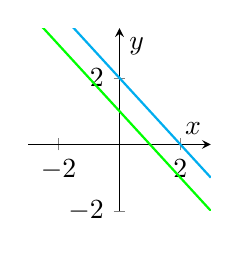
\begin{tikzpicture}
                \begin{axis}[
                    axis lines = middle,
                    xlabel = {$x$},
                    ylabel = {$y$},
                    xmin = -3, xmax = 3,
                    ymin = -2, ymax = 3.5,
                    samples = 10,
                    domain = -3:3,
                    width = 3.9cm,
                    height = 3.9cm
                ]
                    \addplot[color=green, thick] {1-x};
                    \addplot[color=cyan, thick] {2-x};
                \end{axis}
            \end{tikzpicture}

            Lösungsmenge\\
            $L = \emptyset$
        \end{center}
        
    \end{minipage}
    \begin{minipage}{3.9cm}
        \begin{center}
            \begin{equation*}
                \begin{split}
                    \hgreen{$x + y = 2$}\\
                    \hcyan{$x - y = 0$}
                \end{split}
            \end{equation*}
            bzw.\\
            \mesk
            $\left(
                \begin{array}{ccc}
                    \rowcolor{green}
                    1 & 1 & 2\\
                    \rowcolor{cyan}
                    1 & -1 & 0
                \end{array}
            \right)$\\
            \mesk
            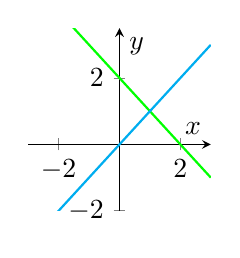
\begin{tikzpicture}
                \begin{axis}[
                    axis lines = middle,
                    xlabel = {$x$},
                    ylabel = {$y$},
                    xmin = -3, xmax = 3,
                    ymin = -2, ymax = 3.5,
                    samples = 10,
                    domain = -3:3,
                    width = 3.9cm,
                    height = 3.9cm
                ]
                    \addplot[color=green, thick] {2-x};
                    \addplot[color=cyan, thick] {x};
                \end{axis}
            \end{tikzpicture}

            Lösungsmenge\\
            $L = \{(1, 1)\}$
        \end{center}
    \end{minipage}
    \begin{minipage}{3.9cm}
        \begin{center}
            \begin{equation*}
                \begin{split}
                    \hgreen{$x + y = 1$}\\
                    \hcyan{$2x + 2y = 2$}
                \end{split}
            \end{equation*}
            bzw.\\
            \mesk
            $\left(
                \begin{array}{ccc}
                    \rowcolor{green}
                    1 & 1 & 1\\
                    \rowcolor{cyan}
                    2 & 2 & 2
                \end{array}
            \right)$\\
            \mesk
            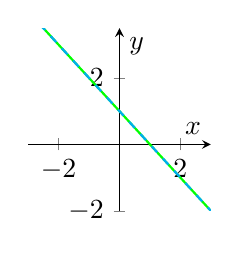
\begin{tikzpicture}
                \begin{axis}[
                    axis lines = middle,
                    xlabel = {$x$},
                    ylabel = {$y$},
                    xmin = -3, xmax = 3,
                    ymin = -2, ymax = 3.5,
                    samples = 10,
                    domain = -3:3,
                    width = 3.9cm,
                    height = 3.9cm
                ]
                    \addplot[color=green, thick] {1-x};
                    \addplot[color=cyan, thick, dashed] {1-x};
                \end{axis}
            \end{tikzpicture}

            Lösungsmenge\\
            $L = \{(t, 1-t) \st t \in \R\}$
        \end{center}
    \end{minipage}
\end{center}

\an{
    Es gibt LGS, aus denen man die Lösungsmenge leicht ablesen kann
}
\ex
\begin{equation*}
    (A \st b) =
    \left(
        \begin{array}{ccccccccc}
            1 & 0 & -7 & 2 & 0 & 1 & 0 & \vline & 0\\
            0 & 1 & 2 & -3 & 0 & -5 & 0 & \vline & 8\\
            0 & 0 & 0 & 0 & 1 & 5 & 0 & \vline & 15\\
            0 & 0 & 0 & 0 & 0 & 0 & 1 & \vline & 42\\
            \rowcolor{cyan}
            0 & 0 & 0 & 0 & 0 & 0 & 0 & \vline & 1
        \end{array}
    \right)\\
\end{equation*}
Ausführlich:
\begin{equation*}
    \begin{split}
        \begin{array}{ccccccccc}
            x_1 &     & -7x_3 & +2x_4 &     & +x_6   &     & = & 0\\
                & x_2 & +2x_3 & -3x_4 &     & -5x_6  &     & = & 8\\
                &     &       &       & x_5 & +5 x_6 &     & = & 15\\
                &     &       &       &     &        & x_7 & = & 42\\
            &&&&&& \cellcolor{cyan}{0} & \cellcolor{cyan}{=} & \cellcolor{cyan}{1}
        \end{array}\\
        \text{\red{Wiederspruch!}}
    \end{split}
\end{equation*}
$\implies L = \emptyset$

\an{
    $L = \emptyset$, falls das LGS eine Gleichung der orm \hcyan{$0 = b_i$ mit $b_i \neq 0$} enthält
}

\newpage
\subsubsection{Zeilenstufenform von LGS}

Allgemein gilt für LGS in \red{Zeilenstufenform} (ZSF):

\begin{equation*}
    (A \st b) =
    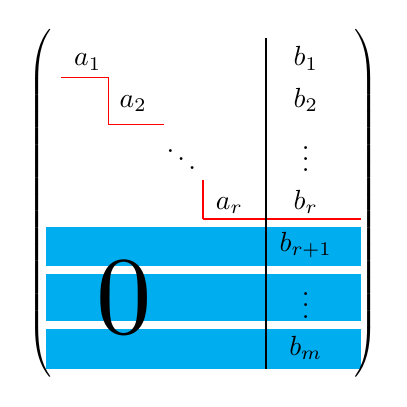
\begin{tikzpicture}[baseline={(current bounding box.center)}]
        \fill[cyan] (-2, -2.1) rectangle (2, -1.6);
        \fill[cyan] (-2, -1.5) rectangle (2, -0.9);
        \fill[cyan] (-2, -0.8) rectangle (2, -0.3);
        
        \matrix (m) [matrix of math nodes,left delimiter={(},right delimiter={)}]{
            a_1 &     &        &     & \smsk & b_1\\
                & a_2 &        &     &       & b_2\\
                &     & \ddots &     &       & \vdots\\
                &     &        & a_r &       & b_r\\
                &     &        &     &       & b_{r+1}\\
                &     &        &     &       & \vdots\\
                &     &        &     &       & b_m\\
        };
        \node at (-1, -1.2) {\scalebox{4}{0}};

        \draw[red] (-1.8, 1.6) -- (-1.2, 1.6);
        \draw[red] (-1.2, 1.6) -- (-1.2, 1);
        \draw[red] (-1.2, 1) -- (-0.5, 1);
        \draw[red] (0, 0.3) -- (0, -0.2);
        \draw[red] (0, -0.2) -- (2, -0.2);
        \draw[black] (0.8, -2.1) -- (0.8, 2.1);
    \end{tikzpicture}
    \text{ mit } a_i \neq 0 \text{ für } i = 1, 2, \dots, r
\end{equation*}

\begin{equation*}
    \begin{array}{lcl}
        (A \st b) \text{ ist lösbar} & \iff & b_{r+1} = b_{r+2} = \dots = b_m = 0\\
        \\
        (A \st b) \text{ ist nicht lösbar} & \iff &
        \parbox{4.1cm}{
            Es gibt ein $b_i$ mit $b_i \neq 0$ und $i \in \{r+1, r+2, \dots, m\}$
        }
    \end{array}
\end{equation*}

\ex\\
LGS über $\R$ mit einem Parameter $a$:
\begin{equation*}
    (A \st b) =
    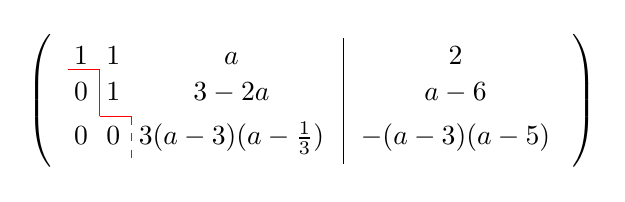
\begin{tikzpicture}[baseline={(current bounding box.center)}]
        \matrix (m) [matrix of math nodes,left delimiter={(},right delimiter={)}]{
            1 & 1 & a                     & \smsk & 2\\
            0 & 1 & 3-2a                  &       & a-6\\
            0 & 0 & 3(a-3)(a-\frac{1}{3}) &       & -(a-3)(a-5)\\
        };
        \draw[black] (0.4, -0.8) -- (0.4, 0.8);

        \draw[red] (-3.1, 0.4) -- (-2.7, 0.4);
        \draw[red] (-2.7, 0.4) -- (-2.7, -0.2);
        \draw[red] (-2.7, -0.2) -- (-2.3, -0.2);
        \draw[red, dashed] (-2.3, -0.2) -- (-2.3, -0.8);
    \end{tikzpicture}
\end{equation*}

\begin{itemize}
    \item 
    $\begin{array}{lcl}
        L = \emptyset & \iff & 3(a-3)(a-\frac{1}{3}) = 0 \text{ und } -(a-3)(a-5) \neq 0\\
                      & \iff & a = \frac{1}{3}
    \end{array}$
    \item $L = \emptyset \iff a \in \R \backslash \{\frac{1}{3}\}$
    
    1. Fall: $a = 3$, unendlich viele Lösungen\\
    2. Fall: $a \in \R \backslash \{\frac{1}{3}, 3\}$, genau eine Lösung
\end{itemize}

\ex
\begin{equation*}
    (A \st b) =
    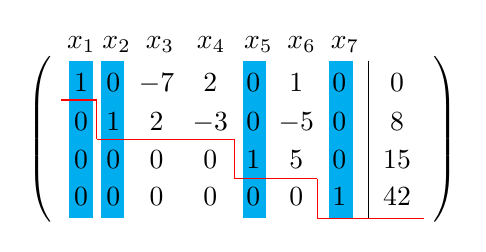
\begin{tikzpicture}[baseline={(current bounding box.center)}]
        \fill[cyan] (-2.2, 1) rectangle (-1.9, -1);
        \fill[cyan] (-1.8, 1) rectangle (-1.5, -1);
        \fill[cyan] (0, 1) rectangle (0.3, -1);
        \fill[cyan] (1.1, 1) rectangle (1.4, -1);

        \matrix (m) [matrix of math nodes,left delimiter={(},right delimiter={)}]{
            1 & 0 & -7 & 2 & 0 & 1 & 0 & \smsk & 0\\
            0 & 1 & 2 & -3 & 0 & -5 & 0 &       & 8\\
            0 & 0 & 0 & 0 & 1 & 5 & 0 &       & 15\\
            0 & 0 & 0 & 0 & 0 & 0 & 1 &       & 42\\
        };

        \node at (-2.05, 1.2) {$x_1$};
        \node at (-1.6, 1.2) {$x_2$};
        \node at (-1.05, 1.2) {$x_3$};
        \node at (-0.4, 1.2) {$x_4$};
        \node at (0.2, 1.2) {$x_5$};
        \node at (0.75, 1.2) {$x_6$};
        \node at (1.3, 1.2) {$x_7$};

        \draw[black] (1.6, 1) -- (1.6, -1);

        \draw[red] (-2.3, 0.5) -- (-1.85, 0.5);
        \draw[red] (-1.85, 0.5) -- (-1.85, 0);
        \draw[red] (-1.85, 0) -- (-0.1, 0);
        \draw[red] (-0.1, 0) -- (-0.1, -0.5);
        \draw[red] (-0.1, -0.5) -- (0.95, -0.5);
        \draw[red] (0.95, -0.5) -- (0.95, -1);
        \draw[red] (0.95, -1) -- (2.3, -1);
    \end{tikzpicture}
    \mesp \text{\cyan{reduzierte} \red{ZSF}}
\end{equation*}

\begin{minipage}{3cm}
    $\begin{array}{lcl}
        x_3 &=& r\\
        x_4 &=& s\\
        x_5 &=& t
    \end{array}$
\end{minipage}
\begin{minipage}{8cm}
    $\begin{array}{lclcl}
        x_1 & = & 7r - 2s - t & = & 7r - 2s - t\\
        x_2 & = & -2r + 3s + 5t & = & 8 - 2r + 3s + 5t\\
        x_5 & = & -5t & = & 15 - 5t\\
        x_7 & = & 42 & = & 42
    \end{array}$
\end{minipage}

$L = \{(\overbrace{7r-2s-t}^{x_1},\overbrace{8-2r+3s+5t}^{x_2},\overbrace{r}^{x_3},\overbrace{s}^{x_4},\overbrace{15-5t}^{x_5},\overbrace{t}^{x_6},\overbrace{42}^{x_7}) \st r,s,t \in \R\}$

\subsection{Elementare Zeilenumformungen}

\begin{itemize}
    \item Vertauschen zweier Zeilen
    \item Multiplikation einer Zeile mit einem Skalar $k \in K \backslash \{0\}$
    \item Addieren des $k$-fachen ($k \in K$) einer Zeile zu einer anderen Zeile
\end{itemize}

\se{Bei Anwendung von elementaren Zeilenumformungen ändert sich die Lösungsmenge des LGS nicht}

\prop{Multiplikation einer Zeile mit einem Skalar $k \in K \backslash \{0\}$ verändert die Lösungsmenge eines LGS nicht}

\pr{
    Das LGS ($S'$) entstehe aus dem LGS ($S$), indem  die erste (da Zeilen beliebig vertauscht werden können, die $i$-te) Zeile mit $k \in K \backslash \{0\}$ multipliziert wird.
    
    \begin{minipage}{5cm}
        LGS ($S$):\\
        $\sum_{j=1}^{n}a_{ij}x_j=b_i$\\
        ($i = 1,2,\dots,m$)
        \vspace{40px}
    \end{minipage}
    \begin{minipage}{5cm}
        LGS ($S'$):\\
        $\sum_{j=1}^{n}a_{ij}x_j=b_i$\\
        ($i = 1,2,\dots,m$)

        mit $a'_{1j} = k \cdot a_{1j}, b'_1 = k \cdot b_1$\\
        und $a'_{ij} = a_{ij}, b'_i = b_i$\\
        \phantom{\mesp}für $j=1,2,\dots,n$\\
        \phantom{\mesp}und $i=2,3,\dots,m$
    \end{minipage}

    Jede Lösung (\hcyan{$l_1, ..., l_n$}) von $S$ erfüllt $\sum_{j=1}^{n}a_{ij}b_j=b_i$ $(i=1,\dots,m)$
    und ist gleichzeitig eine Lösung von $S'$, denn:
    \begin{equation*}
        \sum_{j=1}^{n}a'_{1j}l_j = \sum_{j=1}^{n}\red{k} \cdot a_{1j}l_j = \red{k} \cdot \sum_{j=1}^{n}a_{1j}l_j = \red{k} \cdot b_i = b'_i
    \end{equation*}
    \gray{Probe mit der ersten Gleichung. Alle anderen Gleichungen müssen nicht überprüft werden, da sie übereinstimmen}

    Jede Lösung (\hcyan{$l'_1, ..., l'_n$}) von $S'$ erfüllt $\sum_{j=1}^{n}a_{ij}b_j=b_i$ $(i=1,\dots,m)$
    und ist gleichzeitig eine Lösung von $S$, denn:
    \begin{equation*}
        \sum_{j=1}^{n}a_{1j}l'_j = \sum_{j=1}^{n} \red{\frac{1}{k}} \cdot a'_{ij}  \cdot l'_j = \red{\frac{1}{k}} \cdot \sum_{j=1}^{n}a'_{ij}l'_j = \red{\frac{1}{k}} \cdot b'_i = b_i
    \end{equation*}
}

\subsection{Lößen von LGS nach Gauss/Jordan}

$(A \st b)$ 
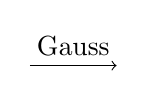
\begin{tikzpicture}
    \draw[->] (0,0) -- (1.1,0) node[midway, above] {Gauss};
\end{tikzpicture}
$\text{\parbox{3.71cm}{LGS in ZSF \\Lösbarkeitsentscheidung}}$
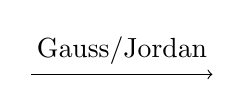
\begin{tikzpicture}
    \draw[->] (0,0) -- (2.3,0) node[midway, above] {Gauss/Jordan};
\end{tikzpicture}
LGS in reduzierter ZSF

\an{
    Spalten dürfen beliebig vertauscht werden, wenn die Bezeichnungen der Unbekannten mitgenommen werden
}
\ex 
\begin{equation*}
    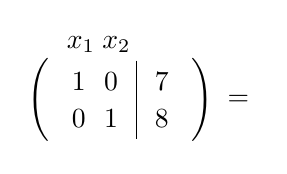
\begin{tikzpicture}[baseline={(current bounding box.center)}]
        \matrix (m) [matrix of math nodes,left delimiter={(},right delimiter={)}]{
            1 & 0 & \mesk & 7\\
            0 & 1 &       & 8\\
        };
        \node at (-0.5, 0.7) {$x_1$};
        \node at (-0.05, 0.7) {$x_2$};
        \draw[black] (0.2, 0.5) -- (0.2, -0.5);
        \node at (1.5, 0) {$=$};
    \end{tikzpicture}
    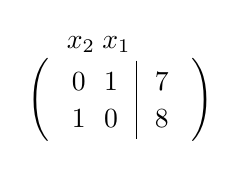
\begin{tikzpicture}[baseline={(current bounding box.center)}]
        \matrix (m) [matrix of math nodes,left delimiter={(},right delimiter={)}]{
            0 & 1 & \mesk & 7\\
            1 & 0 &       & 8\\
        };
        \node at (-0.5, 0.7) {$x_2$};
        \node at (-0.05, 0.7) {$x_1$};
        \draw[black] (0.2, 0.5) -- (0.2, -0.5);
    \end{tikzpicture}
\end{equation*}

\de{Bei dem \red{Eliminationsverfahren nach Gauss} wird das LGS so umgeformt, dass alle Elemente unterhalb der Zeilenstufe Null sind $\implies$ Zeilenstufenform.}

\de{Bei dem \red{Eliminationsverfahren nach Gauß$\backslash$Jordan} wird ein LGS in ZSF mithilfe von Umformungen in die reduzierte ZSF gebracht, sodass sich Lösungen leicht ablesen lassen.}

\newpage
\section{Vektorräume über einem Körper K}

\de{
    Die \red{Lineare Algebra} ist die Theorie der Vektorräume und der Linearen Abbildungen.
}
\de{
    \red{Vektoren} sind Elemente von Vektorräumen.
}
\ex
\begin{itemize}
    \item $\vvec{a}{b}$ mit $a,b \in \R$
    \item $\begin{pmatrix}
        1 & 2 & 3\\
        4 & 5 & 6\\
        7 & 8 & 9
    \end{pmatrix}$
    \item $f: \R \to \R: x \mapsto \ln(x)$ (Logarithmusfunktion)
    \item $\{0,8,15\}$
    \item $\int_{0}^{1} \sin(x)dx$
\end{itemize}

\an{
    Die gemeinsamen Eigenschaften für das Rechnen mit diesen\\
    konkreten mathematischen Objekten werden in der linearen Algebra untersucht.
}
\de{
    Sei $K$ ein Körper. Ein \red{K-Vektorraum} $(V; +; (k \st k \in K))$ besteht aus
    \begin{itemize}
        \item einer nichtleeren Menge $V$
        \item einer Addition $+: V \times V \to V$
        \item einer Skalarmultiplikation $(k \st k \in K): K \times V \to V$
    \end{itemize}
    mit den Eigenschaften $(1)$ bis $(10)$ - die Vektorraumaxiome.

    Die Elemente von $V$ heißen \red{Vektoren}.
}

Abkürzung: VR für Vektorraum

\ex 
\begin{itemize}
    \item $\R$-VR: reeller Vektorraum
    \item $\C$-VR: komplexer Vektorraum
\end{itemize}

\subsection{Vektorraumaxiome}

\begin{enumerate}
    \item Für je zwei Elemente $v_1,v_2 \in V$ ist $v_1 \red{+} v_2$ ein \red{eindeutig bestimmt}es Element von $V$.
    \item $\red{+}$ ist \red{assoziativ}: $(v_1 + v_2) + v_3 = v_1 + (v_2 + v_3)$ für alle $v_1,v_2,v_3 \in V$
    \item $\red{+}$ ist \red{kommutativ}: $v_1 + v_2 = v_2 + v_1$ für alle $v_1,v_2 \in V$
    \item $\red{+}$ hat ein \red{neutrales Element} $0$: $v + 0 = v$ für alle $v \in V$
    \item Jedes Element $v \in V$ hat ein \red{inverses Element} $-v$ bezüglich $\red{+}$: $v + (-v) = 0$
    \item Für jedes $k \in K$ und jedes $v \in V$ ist $\red{kv}$ ein \red{eindeutig bestimmt}es Element von $V$.
    \item Es gilt: $\red{1v = v}$ für alle $v \in V$
    \item Es gilt: $\red{(k_1k_2)v = k_1(k_2v)}$ für alle $k_1,k_2 \in K$ und alle $v \in V$
    \item Es gilt: $\red{(k_1 + k_2)v = k_1v + k_2v}$ für alle $k_1,k_2 \in K$ und alle $v \in V$
    \item Es gilt: $\red{k(v_1 + v_2) = kv_1 + kv_2}$ für alle $k \in K$ und alle $v_1,v_2 \in V$
\end{enumerate}

\an{
    Die Axiome $(1)$ bis $(10)$ enthalten keinen Widerspruch, da es Modelle (Beispiele für VR) gibt, die diese Axiome erfüllen.
}

\ex \begin{itemize}
    \item Körper sind Vektorräume über sich selbst: $\R$-VR, $\C$-VR, $GF(2)$-VR
    \item Sei $K$ ein Körper. $K^{m \times n}$ mit der Matrizenaddition und der Skalarmultiplikation von Matrizen bildet einen $K$-VR mit dem Nullvektor $\mathbf{0}_{m \times n}$ (Nullmatrix)
    \item $R^n := R^{n \times 1} = \{\vvvec{a_1}{\vdots}{a_n} \st a_1,\dots,a_r \in \R\}$\\
    $\C^n := \C^{n \times 1}$\\
    $GF(2)^n := GF(2)^{n \times 1}$\\
    sind spezielle VR $K^n := K^{n \times 1}$ (VR der \underline{Spaltenvektoren})\\
    $\begin{pmatrix}
        0\\
        0\\
        \vdots\\
        0
    \end{pmatrix}$ ist der Nullvektor
    \item $\R$-VR $R^2$: $\overbrace{\underbrace{\{\vvec{a}{b} \mid a,b \in \R\}}_{\text{Trägermenge}}; \underbrace{+, (k \mid k \in \R)}_{\text{Operationssymbole}}}^{\text{Trägermenge}}$
    \item Sei $A$ eine nichtleere Menge und $K$ ein Körper.\\
    Der VR der Abbildungen ist $f: A \to K$ mit\\
    \mesp Addition: $f_1 + f_2: x \mapsto f_1(x) + f_2(x)$\\
    \mesp Skalarmultiplikation: $kf: x \mapsto k \cdot f(x)$\\
    $f: A \to K: a \mapsto 0_K$ ist der Nullvektor
    \item Sei $A$ eine nichtleere Menge und $K = GF(2)$.
    \item Die Potenzmenge $P(A) := \{X \st X \subseteq A\}$ mit der\\
    \mesp Addition: $X + Y := X \xor Y = (X \backslash Y) \cup (Y \backslash X)$\\
    \mesp Skalarmultiplikation: $1X := X$, $0X := \emptyset$\\
    bildet einen $GF(2)$-VR mit dem Nullvektor $\emptyset$
\end{itemize}

\an{
    Nullvektor $0_v$ und Nullelement des Körpers $0_k$ sind eindeutig bestimmt.
}
\pr{
    Seien $0_{v_1}$ und $0_{v_2}$ Nullvektoren von $V$.
    Dann gilt:\\
    \mesp $0_{v_1} + 0_{v_2} = 0_{v_1}$ (da $0_{v_2}$ Nullvektor)\\ 
    \mesp $0_{v_1} + 0_{v_2} = 0_{v_2}$ (da $0_{v_1}$ Nullvektor)

    Also gilt: $0_{v_1} = 0_{v_2}$

    Analog für $0_k$.
}

\subsubsection{Rechenregeln für VR}

\begin{itemize}
    \item $kv = 0_v \iff k = 0$ oder $v = 0$ für alle $k \in K, v \in V$
    \item $(-k)v = -kv$ für alle $k \in K, v \in V$\\
    Insbesondere gilt: $(-1)v = -v$ für alle $v \in V$
\end{itemize}

\subsection{Untervektorräume}

\de{
    \red{Unterstrukturen} sind Teilmengen eines Grundraumes, die die gleichen Eigenschaften haben wie dieser Grundraum.
}
\de{
    Sei $V$ ein $k$-VR und $U \subseteq V$.\\
    $U$ heißt \red{Untervektorraum} (UVR) von $V$, wenn gilt:
    \begin{itemize}
        \item $0_v \in U$
        \item $U$ ist abgeschlossen bezüglich $+$: $a, b \in U \implies a + b \in U$
        \item $U$ ist abgeschlossen bezüglich der Skalarmultiplikation:\\
        $a \in U, k \in K \implies ka \in U$
    \end{itemize}
}
\an{
    Jeder UVR von $V$ erfüllt die Vektorraumaxiome und bildet daher selbst einen $K$-VR.
}

\ex Sei $V$ ein $K$-VR. Dann gilt:
\begin{itemize}
    \item $\{0_v\}$ ist ein UVR von $V$ und wird \red{Nullraum} genannt.
    \item $V$ ist ein UVR von $V$.
\end{itemize}

\ex $V = \R^3$

$U_1 = \{\vvvec{0}{0}{0}\}$ (Nullraum) ist ein UVR von $\R^3$

$U_2 = \{\vvvec{a}{0}{0} \st a \in \R\}$ ist ein UVR von $\R^3$

\se{
    Seien $U_1$ und $U_2$ UVR des VR $V$. Dann ist auch $U_1 \cap U_2$ ein UVR von $V$.
}
\pr{
    Wegen $U_1 \subseteq V, U_2 \subseteq V$ gilt auch $U_1 \cap U_2 \subseteq V$:
    \begin{itemize}
        \item Wegen $0_v \in U_1, 0_v \in U_2$ gilt auch $0_v \in U_1 \cap U_2$
        \item Seien $a,b \in U_1 \cap U_2$. Dann gilt $a,b \in U_1$ und $a,b \in U_2$.
        
        Weil $U_1, U_2$ abgeschlossen bzgl. $+$ sind, gilt\\
        $a + b \in U_1, a+b \in U_2$. Dann gilt auch $a,b \in U_1 \cap U_2$.

        d.h. $U_1 \cap U_2$ ist abgeschlossen bzgl. $+$.
        \item Analog zeigt man:\\
        $U_1 \cap U_2$ ist abgeschlossen bzgl. der Skalarmultiplikation.
    \end{itemize}
}

\newpage
\subsection{Spannräume}
\de{
    Sei $V$ ein VR und $T \subseteq V$.\\
    Den kleinsten UVR $U$ von $V$ mit $T \subseteq U$ nennt man den \red{Spannraum $Span(T)$} von $V$
}
\an{Der Spannraum $Span(T)$ wird auch kurz mit $\spann{T}$ bezeichnet.}
\ex 

Span($\{\vvec{-2}{-4}, \vvec{1}{2}, \vvec{2}{4}\}$) = $\spann{\{\vvec{-2}{-4}, \vvec{1}{2}, \vvec{2}{4}\}} = \{\vvec{t}{2t} \st t \in \R\}$

\an{
    \begin{itemize}
        \item Span$(V) = \spann{V} = V$
        \item Span$(\emptyset) = \spann{\emptyset} = \{0_v\}$ \red{(Nullraum)}\\
        \gray{Das Nullelement ist immer im Spannraum. Es gilt, dass $T \subseteq U$ für alle UVR U von V gilt.}
    \end{itemize}
}

\de{
    Sei $V$ ein $K$-VR, $v_1,\dots,v_n \in V$ und $k_1, \dots, k_n \in K$.\\
    Dann nennt man $k_1v_1, \dots, k_nv_n$ eine \red{Linearkombination} (LK)\\
    der Vektoren $v_1, \dots, v_n$ mit den Koeffizienten $k_1, \dots, k_n$
}
\an{
    Jeder UVR von $V$, der $v_1, \dots, v_n$ enthält, enthält auch sämtliche Linearkombinationen von $v_1, \dots, v_n$ mit Koeffizienten uas $K$.

    Seien $v_1, \dots, v_n \in V$. Dann ist\\
    $U := \{k_1,v_1 + \dots + k_nv_n \st k_1, \dots, k_n \in K\}$ der kleinste UVR von $V$
    \begin{itemize}
        \item $U \subseteq V$
        \item $0_kv_1 + \dots + 0_kv_n = 0_v \in U$
        \item $U$ ist abgeschlossen bzgl. $+$
        \item $U$ ist abgeschlossen bzgl. Skalarmultiplikation
    \end{itemize}
}

Sei $V$ ein $K$-VR und $T := \{v_1, \dots, v_n\} \subseteq V$\\
Dann gilt: Span$(T) = \{k_1, v_1 + \dots + k_nv_n \st k_1, \dots, k_n \in K\}$

\ex $V = \R^2$

Span$(\{\vvec{-2}{-4}, \vvec{1}{2}, \vvec{2}{4}\}) = \{a \vvec{-2}{-4} + b \vvec{1}{2} + c \vvec{2}{4} \st a,b,c \in \R\}$

\newpage
\ex $V = \R^3$

$U := \{\vvvec{2a}{a+b}{b} \st a,b \in \R\}$ ist ein UVR von $R^3$.

\pr{
    $U = \{a \vvvec{2}{1}{0} + b \vvvec{0}{1}{1} \st a,b \in \R\} =$ Span$(\underbrace{\{\vvvec{2}{1}{0}, \vvvec{0}{1}{1}\}}_{\subseteq \R^3})$

    Ein Spannraum ist nach Definition ein UVR. Also ist $U$ ein UVR von $\R^3$.
}

\subsection{Erzeugendensysteme}

\de{
    Sei $V$ ein $K$-VR, $T \subseteq V$ und $V =$ Spann$(T)$.\\
    Dann nenne man T ein \red{Erzeugendensystem} von $V$
}

\an{
    Jeder Vektorraum $V$ hat ein Erzeugendensystem.\\
    \ex Spann$(V) = V$
}

\an{
    Um einen VR zu beschreiben genügt es, für diesen VR ein Erzeugendensystem anzugeben.
    \begin{itemize}
        \item VR sind durch Angabe eines Erzeugendensystems eindeutig bestimmt.
        \item Für jeden VR $V$ gibt es Erzeugendensysteme $T_1, T_2$ mit $T_1 \neq T_2$.
    \end{itemize}
    Sinnvoll ist es, möglichst kleine Erzeugendensysteme für einen Vektorraum anzugeben.
}

\newpage
\ex $T = \{\vvvec{1}{0}{0}, \vvvec{1}{1}{0}, \vvvec{1}{2}{0}, \vvvec{1}{0}{1}\}$
\begin{itemize}
    \item $T \subseteq \R^3$ \mesp $(\implies \spann{T} \subseteq \R^3)$
    \item Jeder Vektor $\vvvec{a}{b}{c} \in \R^3$ lässt sich als LK von Vektoren aus $T$ darstellen, denn das LGS mit der erweiterten Koeffizientenmatrix
    \begin{equation*}
        (A \st b) =
        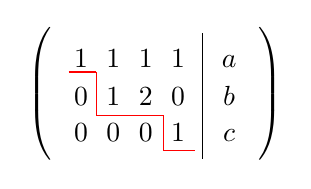
\begin{tikzpicture}[baseline={(current bounding box.center)}]
            \matrix (m) [matrix of math nodes,left delimiter={(},right delimiter={)}]{
                1 & 1 & 1 & 1 & \smsk & a\\
                0 & 1 & 2 & 0 &       & b\\
                0 & 0 & 0 & 1 &       & c\\
            };
            \draw[black] (0.6, -0.8) -- (0.6, 0.8);
    
            \draw[red] (-1.1, 0.3) -- (-0.75, 0.3);
            \draw[red] (-0.75, 0.3) -- (-0.75, -0.25);
            \draw[red] (-0.75, -0.25) -- (0.1, -0.25);
            \draw[red] (0.1, -0.25) -- (0.1, -0.7);
            \draw[red] (0.1, -0.7) -- (0.5, -0.7);
        \end{tikzpicture}
        \text{ ist lösbar } (\implies \R^3 \subseteq \spann{T})
    \end{equation*}
    Also gilt: $\R^3 =$ Span$(\{\vvvec{1}{0}{0}, \vvvec{1}{1}{0}, \vvvec{1}{2}{0}, \vvvec{1}{0}{1}\})$

    d.h $T$ ist ein Erzeugendensystem von $\R^3$.
\end{itemize}

\subsection{Lineare Unabhängigkeit}

\de{
    Sei $V$ ein $K$-VR.\\
    Vektoren $v_1, \dots, v_n \in V$ heißen \red{linear unabhängig}, wenn gilt:
    \[
        \forall k1, \dots, k_n \in K: k_1v_1 + \dots + k_nv_n = 0_v \implies k_1 = \dots = k_n = 0_k
    \]
    Andernfalls heißen diese Vektoren \red{linear abhängig}.
}

\an{
    Man spricht auch von linear unabhänhigen bzw. linear abhängigen Mengen ($\{v_1, \dots, v_n\}$) bzw. Folgen von Vektoren ($(v1, \dots, v_n)$, bei Folgen ist die Reihenfolge ist wichtig).
}
\an{
    Sei $V$ ein $K$-VR.\\
    Vektoren $v_1, \dots, v_n \in V$ sind linear abhängig, wenn gilt:
    \[
        \exists k1, \dots, k_n \in K: k_1v_1 + \dots + k_nv_n = 0_v \land \exists i \in \{1, \dots, n\}: k_i \neq 0_k
    \]
    Ist $(k_i \neq 0)$, so kann die Gleichung nach $v_i$ aufgelöst werden.\\
    Somit ist $v_i$ eine Linearkombination der anderen Vektoren.
}

\an{
    Sei $V$ ein $K$-VR.\\
    Für beliebige Vektoren $v_1, \dots, v_n \in V$ gilt:
    \begin{itemize}
        \item Sind $v_1, \dots, v_n$ linear unabhängig, dann gibt es nur eine Linearkombination dieser Vektoren, die den Nullvektor ergibt:
        \[
            0_kv_1 + \dots + 0_kv_n = 0_v
        \]
        \item Sind $v_1, \dots, v_n$ linear abhängig, dann gibt mindestens zwei verschiedene Linearkombinationen dieser Vektoren, die den Nullvektor ergeben:
        \[
            \begin{split}
                0_kv_1 + \dots + 0_kv_n &= 0_v\\
                k_1v_1 + \dots + k_nv_n &= 0_v
            \end{split}
        \]
        mit $-k_iv_i = k_1v_1 + \dots + k_{i-1}v_{i-1} + k_{i+1}v_{i+1} + \dots + k_nv_n$
    \end{itemize}
}
\ex $V = \R^3$
\begin{itemize}
    \item $\vvvec{1}{0}{0}, \vvvec{1}{1}{0}, \vvvec{2}{2}{0}$ sind linear abhängige Vektoren,\\
    denn $0 \vvvec{1}{0}{0} + 2 \vvvec{1}{1}{0} + (-1) \vvvec{2}{2}{0} = \vvvec{0}{0}{0}$
    \item $\vvvec{1}{0}{0}, \vvvec{1}{1}{0}, \vvvec{1}{1}{1}$ sind linear unabhängige Vektoren,\\
    denn $k_1 \vvvec{1}{0}{0} + k_2 \vvvec{1}{1}{0} + k_3 \vvvec{1}{1}{1} = \vvvec{0}{0}{0} \implies k_1 = k_2 = k_3 = 0$
\end{itemize}
\an{
    Für jeden $K$-VR $V$ mit $v_1,v_2 \in V$ gilt:\\
    $v_1,v_2$ sind linear abhängig $\iff \exists k \in K: v_2 = kv_1$
}
\pr{
    $(\implies): v_1, v_2$ linear abhängig\\
    $\implies \exists k_1,k_2 \in K: k_1v_1 + k_2v_2 = 0_v \land (k_1,k_2) \neq (0,0)$
    O.B.d.A sei $k_2 \neq 0_k$.\\
    Dann gilt: $k_1v_1 + k_2v_2 = 0_v$
    \begin{align*}
        &\implies \textcolor{red}{-k_1v_1} + k_1v_1 + k_2v_2 &=& \textcolor{red}{-k_1v_1} + 0_V \\
        &\implies k_2v_2 &=& -k_1v_1\\
        &\implies v_2 &=& \frac{-k_1}{k_2}v_1
    \end{align*}
    D.h. $v_2 = kv_1$ mit $k = \frac{-k_1}{k_2}$

    $(\impliedby):$ Sei $v_2 = kv_1$. Dann gilt:\\
    $kv_1 + (-1)v_2 = kv_1 + (-1)kv_1 = kv_1 + (-k)v_1 = (k+ (-k))v_1 = 0_Kv_1 = 0_V$ und $(k,-1) \neq (0,0)$.

    Also sind $v_1,v_2$ linear abhängig.
}

\an{
    Für jeden $K$-VR $V$ gilt: $\emptyset$ ist linear unabhängig.
}

\an{
    Für jeden $K$-VR gilt: $0_v$ ist linear abhängig. Insbesondere ist jede Menge, die $0_v$ enthält, linear abhängig.\\
    \pr{
        $1 \cdot 0_v = 0_k0_v$\\
        Es gilt sogar: $k0_v = 0_v$ für alle $k \in K$ und $|K| > 1$
        }
}

\subsection{Basis und Dimension von Vektorräumen}

\de{
    Sei $V$ ein $K$-VR und $B \subseteq V$.\\
    $B$ heißt eine \red{Basis} von $V$, wenn gilt:
    \begin{itemize}
        \item $B$ ist linear unabhängig
        \item $V =$ Span$(B)$ = $\spann{B}$
    \end{itemize}
}

\an{
    $\{
        \begin{pmatrix}
            1\\
            0\\
            \vdots\\
            0
        \end{pmatrix},
        \begin{pmatrix}
            0\\
            1\\
            \vdots\\
            0
        \end{pmatrix},
        \dots,
        \begin{pmatrix}
            0\\
            0\\
            \vdots\\
            1
        \end{pmatrix}
    \}$ ist die \red{Standardbasis} von $K^n$.
}

\an{
    Der Nullraum hat als Basis die leere Menge:
    \[
        \{0_v\} = \spann{\emptyset} \quad B = \emptyset    
    \]
}

\newpage
\ex
\begin{itemize}
    \item $\R^3$ hat die Standardbasis $\{\vvvec{1}{0}{0}, \vvvec{0}{1}{0}, \vvvec{0}{0}{1}\}$.
    \item Für $\R$ ist $\{1\}$ eine Basis. Aber auch $\{-1\}, \{\pi\}$ usw. sind Basen von $\R$. $\{0\}$ ist keine Basis von $\{\R\}$
    \item Der $\R$-VC $\C$ hat als Basis $\{1, i\}$
    \item $R^{2 \times 2}$ hat als Basis $\{
        \begin{pmatrix}
            1 & 0\\
            0 & 0
        \end{pmatrix},
        \begin{pmatrix}
            0 & 1\\
            0 & 0
        \end{pmatrix},
        \begin{pmatrix}
            0 & 0\\
            1 & 0
        \end{pmatrix},
        \begin{pmatrix}
            0 & 0\\
            0 & 1
        \end{pmatrix}
    \}$.
    \item Der $GF(2)$-VR $P(A)$ mit $A = \{1, \dots, n\}$ hat als Basis\\
    $\{\{1\}, \{1,2\},\dots, \{1,\dots,n\}\}$ bzw. $\{\{1\},\{2\},\dots,\{1,\dots,n\}\}$ 
\end{itemize}

\an{
    Sei $V$ ein $K$-VR und $B$ eine Basis von $V$.\\
    Dann gilt:
    \begin{itemize}
        \item $B$ ist ein \red{minimales Erzeugendensystem} von V:
        \begin{itemize}
            \item $B$ ist ein Erzeugendensystem von $V$
            \item Jede echte Teilmenge von $B$ ist kein Erzeugendensystem von $V$
        \end{itemize}
        \item $B$ ist eine \red{maximale linear unabhängige Teilmenge} von $V$:
        \begin{itemize}
            \item $B$ ist linear unabhängig
            \item Durch $B \cup \{v\} \; (v \in V, v \notin B)$ erhält man eine linear abhängige Menge.
        \end{itemize}
    \end{itemize}
}

\subsubsection{Dimension eines VR}

\se{
    Je zwei Basen eines endlichen Vektorraums haben die gleiche Anzahl von Elementen.
}
\de{
    Hat ein VR $V$ eine Basis $B$ mit $|B|=n$, dann wird die Anzahl der Basiselemente dieses VR die \red{Dimension $\dim(V)$} von $V$ genannt:
    \[
        \dim(V) = n
    \]
}
\ex \begin{itemize}
    \item $\dim(\R^n) = \dim(\C^n) = \dim(GF(2)^n) = \dim(K^n) = n$
    \item $\dim(K^{m \times n}) = m \cdot n$
\end{itemize}

\newpage
\an{
    Ein Beispiel für einen unendlich-dimensionalen VR ist die reelle Polynomfunktion:
    \[
        f: \R \to \R: x \mapsto a_0 + a_1x + a_2x^2 + \dots + a_nx^n
    \]
}

\section{Kern und Rang von Matrizen}

\subsection{Kern von Matrizen}

\de{
    Sei $K$ ein Körper und $A \in K^{m \times n}$.\\
    \red{$\ker(A)$} $:= \{x \st x \in K^n, Ax = 0_{K^m}\}$ heißt \red{Kern der Matrix}.
}

\an{
    Der Kern einer Matrix ist ein UVR von $K^n$.
}

\subsubsection{Kern eines homogenen LGS}

\an{
    Die Lösungsmenge eines homogenen LGS ist ein VR:
    \[
        L\text{*} = \{x \st x \in K^n, Ax = 0_{K^m}\}   
    \]
}
\ex $A = \begin{pmatrix}
    1 & 1 & 1\\
    1 & -1 & 1\\
    1 & 0 & 1
\end{pmatrix} \to \begin{pmatrix}
    1 & 1 & 1\\
    0 & -2 & 0\\
    0 & -1 & 0
\end{pmatrix} \to \begin{pmatrix}
    1 & 0 & 1\\
    0 & 1 & 0
\end{pmatrix}$

$x_3 = t \in \R \quad x_2 = 0 \quad x_1 = -t$

\[
    \ker(A) = L\text{*} = \{\vvvec{-t}{0}{t} \st t \in \R\} = \{t \vvvec{-1}{0}{1} \st t \in \R\} = \spann{\{\vvvec{-1}{0}{1}\}}
\]
$\{\vvvec{-1}{0}{1}\}$ ist eine Basis von $\ker(a)$; $\dim(\ker(A)) = 1$

\newpage
\subsubsection{Kern eines inhomogenen LGS}

Inhomogenes LGS: $A_{m \times n} \cdot x_{n \times 1} = b_{m \times 1} \neq 0_{m \times 1}$

Lösungsmenge: $L = \{x \st x \in K^n, Ax = b\} \subseteq K^n$

\an{
    $L$ ist kein UVR von $K^n$, denn $0_{K^n} \notin L$
}
\an{
    \begin{enumerate}
        \item Die Summe einer Lösung des inhomogenen LGS und einer\\
        Lösung des homogenen LGS ist wieder eine Lösung des inhomogenen LGS.
        \item Je zwei Lösungen des inhomogenen LGS unterscheiden sich um eine Lösung des homogenen LGS.
    \end{enumerate}

    Sei $L$ die Lösungsmenge von $ax = b$,\\
    \phantom{Sei} $L*$ die Lösungsmenge von $Ax = 0_{K^m}$,\\
    \phantom{Sei} $x_1$ eine Lösung von $Ax = b$

    Dann gilt:
    \[
        L = \{x_1 + x\text{*} \st x\text{*} \in L\text{*}\} \text{ oder } L = x_1 + L\text{*}
    \]
}

\ex\\
$A = \begin{pmatrix}
    1 & 1 & 1\\
    1 & -1 & 1\\
    1 & 0 & 1
\end{pmatrix} \to \begin{pmatrix}
    1 & 1 & 1\\
    0 & -2 & 0\\
    0 & -1 & 0
\end{pmatrix} \to \begin{pmatrix}
    1 & 0 & 1\\
    0 & 1 & 0
\end{pmatrix}$, $b = \vvvec{3}{1}{2}$

$Ax = b$ hat die Lösungsmenge
\[
    L = \vvvec{1}{1}{1} + \{\vvvec{-1}{0}{1} t \st t \in \R\} = \vvvec{1}{1}{1} + L\text{*} = \vvvec{1}{1}{1} + \ker(A)
\]

\subsection{Affine Teilräume}

\de{
    Sei $V$ ein $K$-VR, $U$ ein UVR von $V$, $v \in V$.\\
    $T := v + U = \{v + u \st u \in U\}$ heißt \red{affiner Teilraum} von $V$.\\
    $\dim(T) := \dim(U)$ heißt Dimension des affinen Teilraums.
}

\an{
    \vspace{-15px}
    \begin{align*}
        v + U \text{ ist ein UVR von} V &\iff v \in U\\
        0_v \in v + U &\iff v \in U
    \end{align*}    
}
Lösungsmengen von LGS $Ax = b$ mit $A \in K^{m \times n}$ sind affine Teilräume von $K^n$.

\ex\\
\begin{minipage}{5cm}
    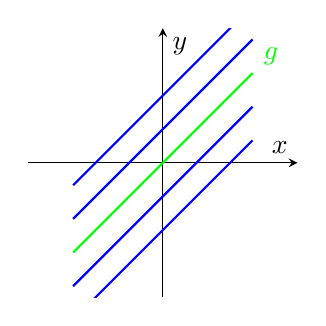
\begin{tikzpicture}
        \begin{axis}[
            axis lines = middle,
            xlabel = {$x$},
            ylabel = {$y$},
            xmin = -6, xmax = 6,
            ymin = -6, ymax = 6,
            samples = 10,
            domain = -4:4,
            width = 5cm,
            height = 5cm,
            xtick=\empty, 
            ytick=\empty
        ]
            \addplot[color=green, thick] {x} node[pos=1.2, anchor=north east] {$g$};
            \addplot[color=blue, thick] {x+1.5};
            \addplot[color=blue, thick] {x-1.5};
            \addplot[color=blue, thick] {x+3};
            \addplot[color=blue, thick] {x-3};
        \end{axis}
    \end{tikzpicture}    
\end{minipage}
\begin{minipage}{5cm}
    Die Menge der Punkte von $g$ ist ein $\underbrace{UVR}_{\text{spezieller affiner Teilraum}}$ von $\R^2$

    Die Menge der Punkte jeder zu $g$ parallelen Geraden bilde einen affinen Teilraum von $R^2$.
\end{minipage}

\de{
    Sei $V$ ein $K$-VR, $\dim(V) = n$.

    \begin{itemize}
        \item $0$-dimensionale affine Teilräume von $V$ heißen \red{Punkte}
        \item $1$-dimensionale affine Teilräume von $V$ heißen \red{Geraden}
        \item $2$-dimensionale affine Teilräume von $V$ heißen \red{Ebenen}
        \item $n-1$-dimensionale affine Teilräume von $V$ heißen \red{Hyperebenen}
    \end{itemize}
}
\ex Hyperebenen in $\R^2$ sind Geraden, in $\R^3$ sind es Ebenen.

\subsection{Rang von Matrizen}

\subsubsection{Spaltenraum}

Sei $A \in K^{m \times n}$, $A = (s_1, s_2,\dots,s_n)$ (Spaltenvektoren von A)
\begin{itemize}
    \item $\col(A) := \spann{\{s_1, s_2,\dots,s_n\}}$ heißt \red{Spaltenraum} von $A$
    \item $\col(A) \in K^m$
    \item $\col(A)$ ist ein UVR von $K^m$
    \item $\dim(\col(A))$ heißt \red{Spaltenrang} von $A$
\end{itemize}

\an{
    Der Spaltenrang von $A$ ist die Maximalzahl linear unabhängiger Spaltenvektoren von $A$.
}

\newpage
\subsubsection{Zeilenraum}

Sei $A \in K^{m \times n}$, $A = \begin{pmatrix}z_1 \\ z_2 \\ \vdots \\ z_m\end{pmatrix}$ (Zeilenvektoren von A)

\begin{itemize}
    \item $\row(A) := \spann{\{z_1, z_2,\dots,z_m\}}$ heißt \red{Zeilenraum} von $A$
    \item $\row(A) \subseteq K^n$
    \item $\row(A)$ ist ein UVR von $K^n$
    \item $\dim(\row(A))$ heißt \red{Zeilenrang} von $A$
\end{itemize}

\an{
    Der Zeilenrang von $A$ ist die Maximalzahl linear unabhängiger\\
    Zeilenvektoren von $A$.
}

\se{
    Für jede Matrix $A$ gilt:
    \[
        \dim(\col(A)) = \dim(\row(A)) 
    \]
}

\subsubsection{Rang einer Matrix}

\de{
    Sei $K$ ein Körper und $A \in K^{m \times n}$. Dann nennt man
    \[
        \rg(A) := \dim(\col(A)) = \dim(\row(A)) 
    \]
    den \red{Rang} von $A$.
}

\an{
    $A \in K^{m \times n} \implies \rg(A) \leq \min(m,n)$
}

\ex $A_1 =\begin{pmatrix}
    1 & 1 & 0\\
    1 & 0 & 0\\
    0 & 0 & 1
\end{pmatrix} \in \R^{3 \times 3}$

$A_1$ hat den Spaltenrang $\dim(\spann{\{\vvvec{1}{1}{0},\vvvec{1}{0}{0},\vvvec{0}{0}{1}\}}) = 3$

$A_1$ hat den Zeilenrang $\dim(\spann{\{(1,1,0),(1,0,0),(0,0,1)\}}) = 3$

$\rg(A_1) = 3$

\newpage
$A_2 = \begin{pmatrix}
    1 & 1 & 0\\
    1 & 0 & 1\\
    0 & 0 & 0 
\end{pmatrix}$

$A_2$ hat den Spaltenrang $\dim(\spann{\{\vvvec{1}{1}{0},\vvvec{1}{0}{0},\gray{\vvvec{0}{0}{0}}\}}) = 2$

$A_2$ hat den Zeilenrang $\dim(\spann{\{(1,1,0),(1,0,1),\gray{(0,0,0)}\}}) = 2$

$\rg(A_2) = 2$

\subsubsection{Rangberechnung für Matrizen}

\an{
    Elementare Zeilenumformungen ändern den Rang einer Matrix nicht.
}

\begin{enumerate}
    \item Bringe die Matrix $A \in K^{m \times n}$ mittels elementarer Zeilenumformungen in Zeilenstufenform
    \item $\rg(A)$ ist die Anzahl der von Null verschiedenen Zeilen in der Zeilenstufenform
\end{enumerate}

\ex
\begin{itemize}
    \item \begin{equation*}
        (A \st b) =
        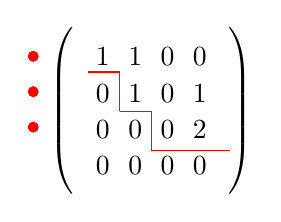
\begin{tikzpicture}[baseline={(current bounding box.center)}]
            \matrix (m) [matrix of math nodes,left delimiter={(},right delimiter={)}]{
                1 & 1 & 0 & 0\\
                0 & 1 & 0 & 1\\
                0 & 0 & 0 & 2\\
                0 & 0 & 0 & 0\\
            };
            \fill[red] (-1.5, 0.7) circle[radius=2pt];
            \fill[red] (-1.5, 0.25) circle[radius=2pt];
            \fill[red] (-1.5, -0.2) circle[radius=2pt];
    
            \draw[red] (-0.8, 0.5) -- (-0.4, 0.5);
            \draw[red] (-0.4, 0.5) -- (-0.4, 0);
            \draw[red] (-0.4, 0) -- (0, 0);
            \draw[red] (0, 0) -- (0, -0.5);
            \draw[red] (0, -0.5) -- (1, -0.5);
                
        \end{tikzpicture}
        \mesp \text{hat den Rang 3}
    \end{equation*}
    \item $\rg(E_n) = n$
    \item $\rg(A) = \rg(A^T)$
\end{itemize}

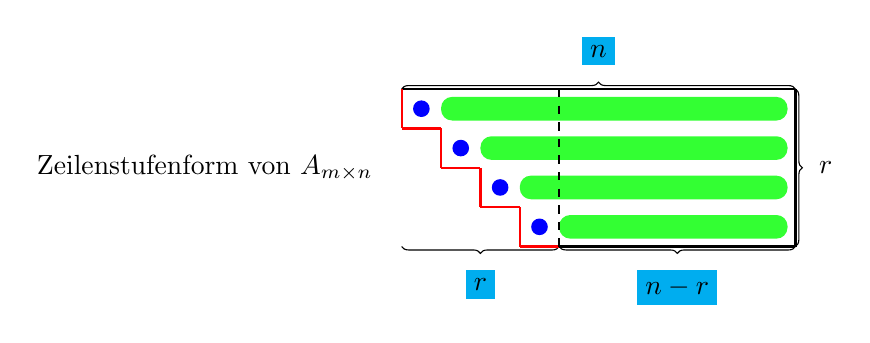
\begin{tikzpicture}

    \node at (-2.5, 1) {Zeilenstufenform von $A_{m \times n}$};

    \draw[thick] (0,2) -- (5,2);
    \draw[decorate, decoration={brace}] (0,2) -- (5,2) node[midway, above=5pt] {\hcyan{$n$}};
    
    \draw[thick] (5,2) -- (5,0);
    \draw[decorate, decoration={brace}] (5,2) -- (5,0) node[midway, right=5pt] {$r$};

    \draw[thick] (5,0) -- (2,0);
    \draw[decorate, decoration={brace}] (5,0) -- (2,0) node[midway, below=5pt] {\hcyan{$n-r$}};

    \draw[decorate, decoration={brace}] (2,0) -- (0,0) node[midway, below=5pt] {\hcyan{$r$}};
    
    \draw[thick, red] (0,2) -- (0,1.5);
    \draw[thick, red] (0,1.5) -- (0.5,1.5);
    \draw[thick, red] (0.5,1.5) -- (0.5,1);
    \draw[thick, red] (0.5,1) -- (1,1);
    \draw[thick, red] (1,1) -- (1,0.5);
    \draw[thick, red] (1,0.5) -- (1.5,0.5);
    \draw[thick, red] (1.5,0.5) -- (1.5,0);
    \draw[thick, red] (1.5,0) -- (2,0);

    \fill[blue] (0.25,1.75) circle[radius=3pt];
    \fill[blue] (0.75,1.25) circle[radius=3pt];
    \fill[blue] (1.25,0.75) circle[radius=3pt];
    \fill[blue] (1.75,0.25) circle[radius=3pt];

    \fill[fill=green!80, rounded corners=4pt] (0.5, 1.9) rectangle (4.9, 1.6);
    \fill[fill=green!80, rounded corners=4pt] (1, 1.4) rectangle (4.9, 1.1);
    \fill[fill=green!80, rounded corners=4pt] (1.5, 0.9) rectangle (4.9, 0.6);
    \fill[fill=green!80, rounded corners=4pt] (2, 0.4) rectangle (4.9, 0.1);

    \draw[dashed, thick] (2, 2) -- (2,0);

\end{tikzpicture}

\begin{itemize}
    \item $r = \rg(A)$ Zeilen
    \item $n-r$ ist die Anzahl der freien Parameter in der Lösungsmenge des homogenen LGS $Ax = 0_{K^m}$\\
    (also $\dim \ker(a) = n-r$)
\end{itemize}

\subsubsection{Dimensionsformel für Matrizen}
\gray{Achtung! Matrizen haben keine Dimension!}

\se{
    \vspace{-15px}
    \[
        A \in K^{m \times n} \implies \rg(A) + \dim\ker(A) = n
    \]
}

\subsection{Lösbarkeitskriterium für LGS}
\[
    Ax = b \text{ lösbar} \iff \rg(A) = \rg(A \st b)
\]

\pr{
    \begin{align*}
        Ax = b \text{ lösbar} &\iff \exists k_1,\dots,k_n \in K \text{ mit } A \cdot \vvvec{k_1}{\vdots}{k_n} = b\\
        &\iff \exists k_1,\dots,k_n \in K \text{ mit } k_1s_1 + \dots + k_ns_n = b\\
        &\iff b \in \col(A)\\
        &\iff \dim(\spann{\{s_1,\dots,s_n\}}) = \dim(\spann{\{s_1,\dots,s_n,b\}})\\
        &\iff \rg(A) = \rg(A \st b)
    \end{align*}
}

\ex
\begin{itemize}
    \item $A = \begin{pmatrix}
        1 & 2 & 3\\
        2 & 4 & 6
    \end{pmatrix}, b_1 = \vvec{4}{8}, b_2 = \vvec{4}{9}$
    \item $\rg(A) = 1, \rg(A \st b_1) = 1, \rg(A \st b_2) = 2$
    \item $Ax = b_1$ ist lösbar, $Ax = b_2$ ist nicht lösbar
\end{itemize}

\subsection{Reguläre Matrizen}

\de{
    Sei $K$ ein Körper.\\
    eine Matrix $A \in K^{n \times n}$ heißt \red{invertierbar}, wenn es eine Matrix $A^{-1} \in K^{n \times n}$ gibt, sodass $A \cdot A^{-1} = A^{-1} \cdot A = E_n$ gilt.\\
    $A^{-1}$ heißt dann die zu $A$ inverse Matrix.
}
\an{
    Invertierbare Matrizen werden auch \red{reguläre Matrizen} genannt.
}

\an{
    Falls die Matrix $A$ invertierbar ist, dann ist $A^{-1}$ eindeutig bestimmt, denn:
}
\[
    A \cdot B = \hgreen{$B \cdot A$} = E_n \land \hcyan{$A \cdot C$} = C \cdot A = E_n
\]
\[
    \implies B = B \cdot \hcyan{$E_n$} = B \cdot \hcyan{$(A \cdot C)$} = \hgreen{$(B \cdot A)$} \cdot C = \hgreen{$E_n$} \cdot C = C
\]

\ex
\begin{itemize}
    \item Die Nullmatrix ist nicht invertierbar:\\
    \pr{
        \vspace{-15px}
        \[
            \text{Für alle Matrizen } A: 0 \cdot A = 0 \neq E_n   
        \]
    }
    \item $E_n^{-1} = E_n$\\
    \pr{
        \vspace{-15px}
        \[
            E_n \cdot E_n = E_n \implies E_n = E_n^{-1}   
        \]
    }
    \item ${(A^{-1})}^{-1} = A$\\
    \pr{
        \vspace{-15px}
        \[
            A^{-1} \cdot A = A \cdot A^{-1} = E_n \implies A = {(A^{-1})}^{-1}
        \]
    }
    \item $(A \cdot B)^{-1} = B^{-1} \cdot A^{-1}$\\
    \pr{
        \vspace{-15px}
        \[
            (A \cdot B) \cdot (B^{-1} \cdot A^{-1}) = A \cdot (B \cdot B^{-1}) \cdot A^{-1} = = A \cdot A^{-1} = E_n
        \]
    }
\end{itemize}

\an{
    Sei $K$ ein Körper und $A \in K^{n \times n}$.\\
    Zur Berechnung von $A^{-1}$ (falls diese Matrix existiert), sind n LGS $Ax = e_i$ zu lösen, wobei $e_i$ der $i$-te Einheitsvektor ist.
}

\newpage
\subsubsection{Paralleles Lösen}

Berechnung von $A^{-1}$ durch paralleles Lösen von $n$ LGS $(A \st e_i)$:
\begin{enumerate}
    \item Notiere \red{$(A \st E_n)$}
    \item Bringe $(A \st E_n)$ mit elementaren Zeilenumformungen in \red{ZSF}
    \item Enthält die umgeformte Matrix $A$ eine \red{Nullzeile}, so existiert $A^{-1}$ nicht.\\
    Andernfalls Bringe die Matrix in die \red{reduzierte ZSF}. Die Matrix hat nun die Form \red{$(E_n \st A^{-1})$}.
\end{enumerate}

\an{
    Für $A = \begin{pmatrix}
        a & b\\
        c & d
    \end{pmatrix} \in \R^{2 \times 2}$ gilt:
    \begin{itemize}
        \item $A$ ist invertierbar $\iff ad - bc \neq 0$
        \item $A$ ist invertierbar $\implies \frac{1}{ad - bc} \begin{pmatrix}
            d & -b\\
            -c & a
        \end{pmatrix}$
    \end{itemize}
}

\subsubsection{Äquivalente Aussagen für invertierbare Matrizen}

Es sei $A \in K^{n \times n}$
\begin{itemize}
    \item $A$ ist eine invertierbare Matrix
    \item $A^T$ ist eine invertierbare Matrix
    \item Die Spaltenvektoren von A sind linear unabhängig
    \item Die Zeilenvektoren von A sind linear unabhängig
    \item $\rg(A) = n$
    \item $\dim \col(A) = n$
    \item $\dim \row(A) = n$
    \item $\dim \ker(A) = 0$
    \item $\ker(A) = \{0_{K^m}\}$
\end{itemize}

\newpage
\section{Lineare Abbildungen}

\de{
    Seien $(V; \oplus_v, (k \st k \in K))$ und $(W; \oplus_w, (k \st k \in K))$ zwei $K$-VR über denselben Körper $K$.\\
    Eine Abbildung $f: V \to W$ heißt \red{lineare Abbildung},\\
    wenn $\forall a,b \in V; k \in K$ gilt:
    \begin{align*}
        f(a \oplus_v b) &= f(a) \oplus_w f(b)\\
        f(k \cdot a) &= k \cdot f(a)
    \end{align*}
    \gray{
        Dies lässt sich auch zu folgender Eigenschaft zusammenfassen:
        $$
            f(a \oplus_v kb) = f(a) \oplus_w kf(b)
        $$
    }
}

\ex \begin{enumerate}
    \item Sei $A \in \R^{m \times n}$. Dann ist $f: \R^n \to \R^m: v \mapsto A \cdot v$ eine lineare Abbildung.
    \pr{
        Seien $v_1,v_2 \in \R^n$ und $k \in \R$. Dann gilt:
        \begin{align*}
            f(v_1 + v_2) &= A \cdot (v_1 + v_2) = A \cdot v_1 + A \cdot v_2 = f(v_1) + f(v_2)\\
            f(k \cdot v_1) &= A \cdot (k \cdot v_1) = k \cdot (A \cdot v_1) = k \cdot f(v_1)
        \end{align*}
    }
    \item Sei $K$ ein Körper und $A \in K^{m \times n}$.\\
    Dann ist $f: K^n \to K^m: v \mapsto Av$ eine lineare Abbildung.
    \item Sei $K$ ein Körper und $k \in K$.\\
    Dann ist $f: K \to K: v \mapsto kv$ eine lineare Abbildung.
\end{enumerate}

\an{
    $f: \R \to \R: x \to mx$ mit $m \in \R$ ist eine lineare Abbildung, aber\\
    $f: \R \to \R: x \to mx + n$ mit $m \in \R, n \in \R \backslash \{0\}$ ist \underline{keine} lineare Abbildung. 
}

\subsection{Eigenschaften linearer Abbildungen}

\begin{enumerate}
    \item Sei $f: V \to W$ eine lineare Abbildung; $v_1, ..., v_n \in V$, $k_1, \dots, k_n \in K$.\\
    Dann gilt:
    $$f(k_1v_1 + \dots + k_nv_n) = k_1 \cdot f(v_1) + \dots + k_n \cdot f(v_n)$$
    \item Sei $f: V \to W$ eine lineare Abbildung und $\{b_1,\dots,b_n\}$ eine Basis von $V$.\\
    Dann gilt:
    \begin{align*}
        f \text{ ist injektiv} &\iff \{f(b_1),\dots,f(b_n)\} \text{ ist linear unabhängig}\\
        f \text{ ist surjektiv} &\iff \spann{\{f(b_1),\dots,f(b_n)\}} = W\\
        f \text{ ist bijektiv} &\iff \{f(b_1),\dots,f(b_n)\} \text{ ist eine Basis von } W
    \end{align*}
\end{enumerate}

\de{
    Seien $V,W$ $K$-VR und $f: V \to W$ eine lineare Abbildung.\\
    $\ker(f) := \{v \in V \st f(v) = 0_W\}$ heißt \red{Kern von $f$}.
}

\an{
    $0_v \in \ker(f)$, denn $f(0_v) = f(0 \cdot 0_v) = 0 \cdot f(0_v) = 0_w$
}

\se{
    Seien $V,W,$ $K$-VR und $f: V \to W$ eine lineare Abbildung.
    $$f \text{ ist injektiv} \iff \ker(f) = \{0_v\}$$
}

\pr{
    ($\implies$) Sei $a \in \ker(f)$.
    \begin{align*}
        &\implies& f(a) &= 0_w \land f(0_v) = 0_w\\
        &\implies& f(a) &= f(0_v)\\
        &\implies& a &= 0_v \text{ (da $f$ injektiv)}\\
        &\implies& \ker(f) &= \{0_v\}
    \end{align*}

    ($\impliedby$) Sei $\ker(f) = \{0_v\}$,\\
    $a,b \in V$ und $f(a) = f(b)$. (zu zeigen: $a = b$)
    \begin{align*}
        &\implies f(a) + (-1 \cdot f(b)) = 1 \cdot f(b) + (-1 \cdot f(b))\\
        &\implies f(a + (-1 \cdot b)) = (1 + (-1)) \cdot f(b) = 0 \cdot f(b) = 0_w\\
        &\implies a + (-1 \cdot b) \in \ker(f) = 0_v\\
        &\implies a + (-1 \cdot b) + 1 \cdot b = 0_v + 1 \cdot b\\
        &\implies a = b 
    \end{align*}
}

\an{
    Sei $f: V \to W$ linear, so ist $\ker(f)$ ein UVR von V
}

\subsubsection{Das Bild linearer Abbildungen}
\de{
    Seien $V,W$ $K$-VR und $f: v \to W$ eine lineare Abbildung.\\
    \red{Im($f$)}$ := \{f(v) \st v \in V\}$ nennt man \red{Bild von $f$}.
}

\an{
    \begin{itemize}
        \item $\im(f) \subseteq W$
        \item $0_w \in \im(f)$, denn $0_v \in V$ und $0_w = f(0_v) \in \im(f)$
    \end{itemize}
}

\an{
    Sei $f: V \to W$ linear, so ist $\im(f)$ ein UVR von $W$
}

\subsubsection{Dimensionsformel für lineare Abbildungen}

\se{
    Seien $V,W$ $K$-VR und $f: V \to W$ eine lineare Abbildung.
    Dann gilt:
    \[
        \dim(V) = n \implies \dim\ker(f) + \dim\im(f) = n
    \]
}

\an{
    Für die lineare Abbildung $f: K^n \to K^m: v \mapsto Av \; (A \in K^{m \times n})$ gilt:
    \begin{align*}
        \ker(f) :&= \{v \in K^n \st f(v) = 0_{K^m}\}\\
        &= \{v \st v \in K, Av = 0_{K^m}\}\\
        &= \ker(A)
    \end{align*}
    Also gilt:
    \[
        \dim \ker(f) = \dim \ker(A)
    \]
    Aus der Dimensionsformel folgt daher wegen $\dim K^n = n$:
    \[
        \dim \im(f) = rg(A)
    \]
}

Sei $A \in \R^{m \times n}$:
\begin{align*}
    \rg(A) = n &\iff \dim \ker(A) = 0\\
    &\iff \ker(A) = \{0_{K^n}\}\\
    &\iff |\ker(A)| = 1\\
    &\iff \text{Es gibt keine freien Parameter}\\
    &\phantom{\iff \;\;} \text{in der Lösungsmenge von } Ax = 0_{K^m}
\end{align*}

\newpage
\an{
    Die lineare Abbildung $f: K^n \to K^m: v \mapsto Av \; (A \in K^{n \times n})$\\
    ist genau dann bijektiv, wenn $\rg(A) = n$ gilt.\\
    Die zu $f$ inverse Abbildung $f^{-1}$ lässt sich mithilfe der zu $A$ inversen Matrix angeben.
}

\ex \begin{itemize}
    \item Die identische Abbildung bildet jeden Vektor auf sich selbst ab:
    $$
    A = \begin{pmatrix}
        1 & 0\\
        0 & 1
    \end{pmatrix}
    $$
    \item Die Nullabbildung bildet jeden Vektor auf den Nullvektor ab:
    $$
    A = \begin{pmatrix}
        0 & 0\\
        0 & 0
    \end{pmatrix}
    $$
    \item Jeder Vektor $(a,b)$ wird auf den doppelten Vektor $(2a,2b)$ abgebildet:
    $$
    A = \begin{pmatrix}
        2 & 0\\
        0 & 2
    \end{pmatrix}
    $$
    \item Senkrechte Projektion auf die x-Achse:
    $$
    A = \begin{pmatrix}
        1 & 0\\
        0 & 0
    \end{pmatrix}
    $$
    \item Senkrechte Projektion auf die Winkelhalbierende des ersten Quadranten:
    $$
    A = \begin{pmatrix}
        \frac{1}{2} & \frac{1}{2}\\
        \frac{1}{2} & \frac{1}{2}
    \end{pmatrix}
    $$
    \item Linksdrehung um den Koordinatenursprung um den Winkel $\varphi$:
    $$
    A = \begin{pmatrix}
        \cos(\varphi) & -\sin(\varphi)\\
        \sin(\varphi) & \cos(\varphi)
    \end{pmatrix}
    $$
    \item Spiegelung an der Geraden, die gegen die $x$-Achse um den Winkel $\varphi$ geneigt ist:
    $$
    A = \begin{pmatrix}
        \cos(\varphi) & \sin(\varphi)\\
        \sin(\varphi) & -\cos(\varphi)
    \end{pmatrix}
    $$
\end{itemize}

\newpage
\an{
    Jede lineare Abbildung ist durch die Bilder der Basisvektoren bereits eindeutig bestimmt:

    Sei $f: V \to W$ linear und $B = \{b_1, \dots, b_n\}$ eine Basis von $V$.\\
    Kennt man $f(b_1), \dots, f(b_n)$, dann kann man für jeden Vektor $v \in V$ das Bild $f(v)$ wie folgt berechnen:

    \begin{itemize}
        \item $v$ als Linearkombination der Basisvektoren darstellen:
        $$v = k_1b_1, \dots, k_nv_n$$
        \item $f(v) = f(k_1b_1 + \dots + k_nv_n) = k_1f(b_1) + \dots + k_nf(b_n)$
    \end{itemize}
}

\subsubsection{Abbildungsmatrizen}

Es sei $f: K^n \to K^m$ eine lineare Abbildung,\\
$(e_1, \dots, e_n)$ die Standardbasis von $K^n$ und $v = \vvvec{v_1}{\vdots}{v_n} \in K^n$.

$f(v) = f(v_1 \cdot \vfec{1}{0}{\vdots}{0} + \dots + v_n \cdot \vfec{0}{0}{\vdots}{1})$\\
\phantom{$f(v)$} $= f(v_1e_1 + \dots + v_ne_n) = v_1 \cdot f(e_1) + \dots + v_n \cdot f(e_n)$\\
\phantom{$f(v)$} $= \underbrace{(f(e_1) \; \dots \; f(e_n))}_A \cdot \vvvec{v_1}{\dots}{v_n} = A \cdot v$ mit $A \in K^{m \times n}$

\de{
    Die Matrix $A$ mit $f(v) = a \cdot v$ für alle $v \in K^n$ heißt \red{Abbildungsmatrix} von $f$.
}

\an{
    \begin{itemize}
        \item Jede Matrix $A \in K^{m \times n}$ bestimmt eine lineare Abbildung:
        $$f_A: K^n \to K^m: x \mapsto A \cdot x$$
        \item Jede lineare Abbildung $f: K^n \to K^m$ wird durch ihre Abbildungsmatrix $A$ eindeutig bestimmt:
        $$A := (f(e_1) \; \dots \; f(e_i) \; f(e_n))$$
        mit $f(x) = A \cdot x$ für alle $x \in K^n$
    \end{itemize}
}

\subsubsection{Darstellungsmatrizen}

$V$ sei ein $K$-VR mit der angeordneten Basis $B = (b_1, \dots, b_n)$\\
$W$ sei ein $K$-VR mit der angeordneten Basis $C = (c_1, \dots, c_m)$\\
$f: V \to W$ sei eine beliebige lineare Abbildung von V in W.

\de{
    \red{$A_{BC}(f)$} nennt man die \red{Darstellungsmatrix} für $f: V \to W$ bezüglich der Basen $B$ und $C$.
}

\an{
    Hat man die Matrix $A_{BC}(f)$ gefunden, dann kann man für Vektoren aus $V$ das Bild $f(v)$ bestimmen, indem man mit Spaltenvektoren rechnet:
    $$A_{BC}(f) \cdot v_B =f(v)_C$$
}

\an{
    Gilt $V = K^n$ und $W = K^m$ für die lineare Abbildung $f: V \to W$ und sind $B,C$ die Standardbasen für $K^n$ bzw. $K^m$, dann ist die Abbildungsmatrix gleich der Darstellungsmatrix $A_{BC}(f)$.
}

\subsubsection*{Aufstellen der Darstellungsmatrix}

\begin{enumerate}
    \item Bestimme $f(b_1) , \dots, f(b_n)$
    \item Stelle $f(b_i)$ mit $i = 1, \dots, n$ bezüglich der Basis $C = (c_1, \dots, c_n)$ dar:
    $$f(b_i) = a_{1i}c_1 + \dots + a_{mi}c_m, \text{ d.h. } f(b_i)_c = \vvvec{a_{1i}}{\vdots}{a_{mi}}$$
    \item Notiere die Darstellungsmatrix $A_{BC}(f)$ von $f$ bzgl. $B,C$:
    $$A_{BC}(f) = \begin{pmatrix}
        a_{11} & \dots & a_{1i} & \dots & a_{1n}\\
        \vdots &  & \vdots &  & \vdots\\
        a_{m1} & \dots & a_{mi} & \dots & a_{mn}
    \end{pmatrix}_{m \times n}$$
\end{enumerate}

\subsubsection*{Berechnung von $f(v)$ mit Hilfe der Darstellungsmatrix $A_{BC}(f)$}

\begin{enumerate}
    \item Stelle $V \in V$ bzgl. der Basis $B = (b_1, \dots, b_n)$ dar:
    $$v = k_1b_1 + \dots + k_nb_n, \text{ d.h. } v_B = \vvvec{k_1}{\vdots}{k_n}$$
    \item Berechne $f(v)$:
    \begin{itemize}
        \item Berechne $a_{BC}(f) \cdot v_B = A_{BC}(f) \cdot \vvvec{k_1}{\vdots}{k_n} = \vvvec{l_1}{\vdots}{l_n} = f(v)_C$
        \item $f(v) = l_1c_1 + \dots + l_mc_m$
    \end{itemize}
\end{enumerate}

Eigenschaften linearer Abbildungen können aus ihrer Darstellungsmatrix abgelesen werden.

\se{
    Sei $f: V \to W$ eine lineare Abbildung mit der Darstellungsmatrix $A := A_{BC}(f) \in K^{m \times n}$. Dann gilt:
    \begin{enumerate}
        \item $v \in \ker(x) \iff v_B \in \ker(A) \iff v_B \in \ker(A_{BC}(f))$
        \item $w \in \im(f) \iff w_C \in \im(f_A)$
    \end{enumerate}
}
\pr{
    Zu $(1)$:\\
    $v \in \ker(f) \iff f(v) = 0_w \iff f(v)_c = 0_{K^m} \iff A \cdot v_B = 0_{K^m} \iff v_B \in Ker(A)$
}

\subsubsection*{Basiswechselmatrix}

\begin{itemize}
    \item Die \red{Basiswechselmatrix $A_{BB'}(id)$} ist die Darstellungsmatrix der linearen Abbildung $id: V \to V: v \mapsto v$, die den Übergang von einer Basis $B$ zu einer Basis $B'$ des $K$-VR $V$ beschreibt.
    \item Ist $B = (b_1, \dots, b_n)$ und $B' = (b_1', \dots, b_n')$, dann gilt:
    $$A_{BB'}(id) = (b_{1B'}, \dots, b_{nB'})$$
    \item Mit der Basiswechselmatrix lassen sich die Koordinaten bezüglich der neuen Basis ausrechnen:
    $$A_{BB'}(id) \cdot v_B = id(v)_{B'} = v_{B'}$$
    \item $A_{BB'}(id)$ ist eine quadratische Matrix und invertierbar.\\
    $A_{BB'}(id)^{-1} = A_{B'B}(id)$ beschreibt den Basiswechsel von $B'$ zurück zu $B$.
\end{itemize}

Für die Basiswechselmatrix gilt:
$$
    \red{A_{BB'}(id) = M(B')^{-1} \cdot M(B)}
$$
Ist $B$ die Standardbasis $(e_1, \dots, e_n)$, dann gilt: $A_{(e_1, \dots, e_n) B'}(id) = M(B')^{-1}$
Ist $B'$ die Standardbasis $(e_1, \dots, e_n)$, dann gilt: $A_{B (e_1, \dots, e_n)}(id) = M(B')$

\section{Determinanten}

\subsection{Eigenschaften von Determinanten}

\an{
    Determinanten sind Abbildungen: $\det: K^{n \times n} \to K: A \mapsto \det(A)$
}

Determinanten sind durch folgende Eigenschaften festgelegt:
\begin{itemize}
    \item det ist mulitlinear, d.h.
    $$
    \det 
    \begin{pmatrix}
        z_1 \\
        \vdots \\
        z_i + k \cdot x \\
        \vdots \\
        z_n
    \end{pmatrix} = det
    \begin{pmatrix}
        z_1 \\
        \vdots \\
        z_i \\
        \vdots \\
        z_n
    \end{pmatrix} + k \cdot det
    \begin{pmatrix}
        z_1 \\
        \vdots \\
        x \\
        \vdots \\
        z_n
    \end{pmatrix}
    $$
    \item det ist alternierend, d.h. hat $A$ zwei gleiche Zeilen, dann gilt $\det(A) = 0$
    \item det ist normiert, d.h. $\det(E_n) = 1$
\end{itemize}

\subsubsection{\texorpdfstring{Berechnung der Determinante für $n = 2$}{Berechnung der Determinante für n = 2}}

\[
    \det \begin{pmatrix}
        a & b\\
        c & d
    \end{pmatrix} = ad - bc
\]

\an{
    $\vvec{a}{b}$ und $\vvec{c}{d}$ linear abhängig $\iff \det \begin{pmatrix}
        a & c\\
        b & d
    \end{pmatrix}$ = 0
}

\pr{
    Ist $\vvec{a}{b} = \vvec{0}{0}$, gilt die Behauptung. Andernfalls:\\
    \underline{Richtung $\implies$:} \begin{align*}
        \vvec{a}{b}, \vvec{c}{d} \text{ lin. abh.} &\implies \exists k \in K \text{ mit } \vvec{c}{d} = k \cdot \vvec{a}{b} = \vvec{ka}{kb}\\
        &\implies \det \begin{pmatrix}
            a & c\\
            b & d
        \end{pmatrix} = det \begin{pmatrix}
            a & ka\\
            b & kb
        \end{pmatrix}\\
        & \hspace{8em} = a \cdot kb - ka \cdot b = 0
    \end{align*}
    \underline{Richtung $\impliedby$:} \begin{align*}
        \det \begin{pmatrix}
            a & c\\
            b & d
        \end{pmatrix} = a \cdot d - b \cdot c = 0 &\implies \vvec{c}{d} = \frac{d}{b} \cdot \vvec{a}{b} \text{ oder }\\
        &\phantom{\implies \text{ }} \vvec{a}{b} = \frac{a}{c} \cdot \vvec{c}{d}\\
    \end{align*}
}

\an{
    $\det(A)$ gibt den Faktor an, um den sich bei der linearen Abbildung $f: x \mapsto Ax$ die "Fläche" von Figuren ändert.
}

\ex $\det \begin{pmatrix}
    0 & 1\\
    2 & 3
\end{pmatrix} = 0 \cdot 3 - 2 \cdot 1 = -2$

\subsubsection{\texorpdfstring{Berechnung der Determinante für $n = 3$}{Berechnung der Determinante für n = 3}}

\[
\det \begin{pmatrix}
    a & b & c\\
    d & e & f\\
    g & h & i
\end{pmatrix} = aei + bfg + cdh - ceg - bdi - afh
\]
\se{
    Der \red{Satz von Sarrus} besagt, dass die Determinante einer $3 \times 3$-Matrix gleich der Differenz der Produkte der Elemente entlang der Haupt- und Nebendiagonalen ist.
}

Die Matrix lässt sich folgendermaßen nach der ersten Zeile entwickeln:
\[
\det \begin{pmatrix}
    a & b & c\\
    d & e & f\\
    g & h & i
\end{pmatrix} = a \cdot \det \begin{pmatrix}
    e & f\\
    h & i
\end{pmatrix} - d \cdot \det \begin{pmatrix}
    b & c\\
    h & i
\end{pmatrix} + g \cdot \det \begin{pmatrix}
    b & c\\
    e & f
\end{pmatrix}
\]

\ex $\det \begin{pmatrix}
    0 & 1 & 2\\
    3 & 4 & 5\\
    6 & 7 & 8
\end{pmatrix} = 0 \cdot 4 \cdot 8 + 3 \cdot 7 \cdot 2 + 1 \cdot 5 \cdot 6 - 6 \cdot 4 \cdot 2 - 7 \cdot 5 \cdot 0 - 3 \cdot 1 \cdot 8 = 0\\
\\
= + 0 \cdot \begin{pmatrix}
    4 & 5\\
    7 & 8
\end{pmatrix} - 1 \cdot \begin{pmatrix}
    3 & 5\\
    6 & 8
\end{pmatrix} + 2 \cdot \begin{pmatrix}
    3 & 4\\
    6 & 7
\end{pmatrix} = 0 - 3 \cdot (-6) + 6 \cdot (-3) = 0$

\de{
    Sei $A \in K^{n \times n}, A = (a_{ij})$.
    \begin{itemize}
        \item Für $n = 1$ gilt: $\det(A) := a_{11}$
        \item Für $n > 1$ gilt: $\det(A) := \sum_{i = 1}^{n}((-1)^{i+1} \cdot a_{i1} \cdot \det(A_i1))$\\
        \gray{Die 1 steht für die Entwicklung nach der 1-ten Spalte}
    \end{itemize}
}

\newpage
\de{
    Die \red{Adjunkte $A_{ij}$} $\in K^{(n-1) \times (n-1)}$ einer Matrix $A \in K^{n \times n}$ ist\\
    diejenige Matrix, die aus $A$ durch Streichen der $i$-ten Zeile und $j$-ten Spalte entsteht.
}

\an{
    Die Vorzeichen erhält man nach der Schachbrettregel:
    $$\begin{pmatrix}
        + & - & + & - & \dots\\
        - & + & - & + & \dots\\
        + & - & + & - & \dots\\
        - & + & - & + & \dots\\
        \vdots & \vdots & \vdots & \vdots & \ddots
    \end{pmatrix}$$
    \gray{Die Vorzeichen wechseln sich entlang der Zeilen ab. Sie sind also \red{alternierend}}
}

\se{
    Entwicklungssatz für Determinanten:

    Sei $A \in K^{n \times n}$ mit $n > 0$ und $A = (a_{ij})$. Dann gilt:
    \[
        \det(A) = \sum_{j = 1}^{n}((-1)^{i+j} \cdot a_{ij} \cdot \det(A_{ij}))
    \]
    $\dots$ ist die Entwicklung nach der $i$-ten Zeile.
    \[
        \det(A) = \sum_{i = 1}^{n}((-1)^{i+j} \cdot a_{ij} \cdot \det(A_{ij}))
    \]
    $\dots$ ist die Entwicklung nach der $j$-ten Spalte.
}

\an{
    In der Definition der Determinante wird nach der $1$-ten Spalte entwickelt.
}

\ex \[
    \det \begin{pmatrix}
        3 & -1 & 0 & -1\\
        -1 & 3 & 0 & -1\\
        -1 & -1 & 0 & 3\\
        0 & 0 & 2 & 1
    \end{pmatrix}
\]

Entwicklung nach der $3$-ten Spalte:
\[
    = - 2 \cdot \det \begin{pmatrix}
        3 & -1 & -1\\
        -1 & 3 & -1\\
        -1 & -1 & 3
    \end{pmatrix} = -2 \cdot 16 = -32
\]

oder Entwicklung nach der $4$-ten Zeile:
\[
    = - 2 \cdot \det \begin{pmatrix}
        3 & -1 & -1\\
        -1 & 3 & -1\\
        -1 & -1 & 3
    \end{pmatrix} + 1 \cdot \begin{pmatrix}
        3 & -1 & 0\\
        -1 & 3 & 0\\
        -1 & -1 & 0
    \end{pmatrix} = -2 \cdot 16 + 1 \cdot 0 = -32
\]

\an{
    Das Berechnen der Deterinanten durch Entwicklung nach\\
    Zeilen/Spalten ist kein effizientes Verfahren, ist bei kleinen oder schwach besetzten Matrizen, also Matrizen mit vielen Nullen, jedoch sinvoll anwendbar.
}

\subsection{Spezielle Determinanten}

\begin{enumerate}
    \item Enthält $A \in K^{n \times n}$ eine Nullzeile oder -spalte, dann gilt $\det(A) = 0$
    \item $det(E_n) = 1$
    \item $\det \begin{pmatrix}
        a_{11} && 0\\
        & \ddots &\\
        0 && a_{nn}
        \end{pmatrix} = 
        \det \begin{pmatrix}
            a_{11} && 0\\
            \vdots & \ddots &\\
            a_{n1} & \dots & a_{nn}
        \end{pmatrix} =
        \det \begin{pmatrix}
            a_{11} & \dots & a_{1n}\\
            & \ddots & \vdots\\
            0 && a_{nn}
        \end{pmatrix}\\
        \\
        = a_{11} \cdot \dots \cdot a_{nn}$
    \item $\det \begin{pmatrix}
        \ddots & \vdots & 0 & 0\\
        \dots & A & 0 & 0\\
        0 & 0 & B & \dots\\
        0 & 0 & \dots & \ddots
    \end{pmatrix} = \det(A) \cdot \det(B)$
    \item $\det(A) = \det(A^T)$
\end{enumerate}

\subsubsection{Umformungsregeln für Determinanten}

\begin{itemize}
    \item Entsteht $B$ aus $A$ durch Vertauschen zweier Spalten/Zeilen, dann gilt $\det(B) = -\det(A)$
    \item Stimmen in $A$ zwei Spalten/Zeilen überein, dann gilt $\det(A) = 0$
    \item Entsteht $B$ aus $A$ durch Multiplikation einer Spalte/Zeile mit $k \in K$, dann gilt $\det(B) = k \cdot \det(A)$
    \item Entsteht $B$ aus $A$, indem man zu einer Spalte/Zeile ein Vielfaches einer anderen Spalte/Zeile addiert, dann gilt $\det(B) = \det(A)$
    \item $\det(k \cdot A) = k^n \cdot \det(A)$ für $A \in K^{n \times n}$
    \item $\det(A \cdot B) = \det(A) \cdot \det(B)$ für $A,B \in K^{n \times n}$
\end{itemize}

\ex \begin{align*}
    \det \begin{pmatrix}
        3 & -1 & -1\\
        -1 & 3 & -1\\
        -1 & -1 & 3
    \end{pmatrix} &= - \det \begin{pmatrix}
        -1 & -1 & 3\\
        -1 & 3 & -1\\
        3 & -1 & -1
    \end{pmatrix}\\
    &= - \det \begin{pmatrix}
        -1 & -1 & 3\\
        0 & 4 & -4\\
        0 & -4 & 8
    \end{pmatrix}\\
    &= - \det \begin{pmatrix}
        -1 & -1 & 3\\
        0 & 4 & -4\\
        0 & 0 & 4
    \end{pmatrix}\\
    &= - (-1) \cdot 4 \cdot 4 = 16
\end{align*}

oder:
\begin{align*}
    \det \begin{pmatrix}
        3 & -1 & -1\\
        -1 & 3 & -1\\
        -1 & -1 & 3
    \end{pmatrix} &= \frac{1}{3} \cdot \det \begin{pmatrix}
        3 & -1 & -1\\
        0 & 8 & -4\\
        -1 & -1 & 3
    \end{pmatrix}\\
    &= \frac{1}{3} \cdot \frac{1}{3} \cdot \det \begin{pmatrix}
        3 & -1 & -1\\
        0 & 8 & -4\\
        0 & -4 & 8
    \end{pmatrix}\\
    &= \frac{1}{3} \cdot \frac{1}{3} \cdot \frac{1}{2} \cdot \det \begin{pmatrix}
        3 & -1 & -1\\
        0 & 8 & -4\\
        0 & 0 & 12
    \end{pmatrix}\\
    &= \frac{1}{3} \cdot \frac{1}{3} \cdot \frac{1}{2} \cdot 3 \cdot 8 \cdot 12 = 16
\end{align*}

\se{
    Der \red{Multiplikationssatz} besagt, dass die Determinante des Produktes von Matrizen gleich dem Produkt der Determinanten der Matrizen ist:
    \[
        \forall A,B \in K^{n \times n}: \det(A \cdot B) = \det(A) \cdot \det(B)
    \]
}

Sei $A \in K ^{n \times n}$ invertierbar, das heißt es existiert ein $A^{-1}$. Dann gilt:
\[
    \det(A^{-1}) = \frac{1}{\det(A)}
\]
\pr{
    \vspace{-3em}
    \begin{align*}
        A \cdot A^{-1} = E_n &\implies \det(A \cdot A^{-1} ) = \det(E_n)\\
        &\implies \det(A) \cdot \det(A^{-1}) = 1\\
        &\implies \det(A^{-1}) = \frac{1}{\det(A)}
    \end{align*}
}

\an{
    Insbesondere gilt: $A \in K^n \times n$ ist genau dann invertierbar, wenn $\det(A) \neq 0$
}

\se{
    Sei $A \in K^{n \times n}$. Dann gilt:
    \begin{align*}
        det(A) \ne 0 &\iff A^{-1} \text{ existiert}\\
        &\iff \rg(A) = n\\
        &\iff \dim \ker(A) = 0\\
        &\iff \ker(A) = \{0_{K^n}\}
    \end{align*}
    \begin{align*}
        det(A) \ne 0 &\iff A^{-1} \text{ existiert nicht}\\
        &\iff \rg(A) < n\\
        &\iff \dim \ker(A) > 0\\
        &\iff \ker(A) \ne \{0_{K^n}\}
    \end{align*}
}

\se{
    Sei $A \in K^{n  \times n}$ und $\det(A) \ne 0$. Dann gilt:
    \[
        A^{-1} = \frac{1}{\det(A)} \cdot ((-1)^{i+j} \cdot \det(A_{ij}))   
    \]
    wobei $A_{ij}$ aus $A$ durch Streichen der $i$-ten Spalte und $j$-ten Zeile entsteht.
}

\newpage
\section{Eigenwerte und Eigenvektoren von Matrizen}

\an{
    Sei K ein Körper und $A \in K^{n \times n}$.\\
    Es gibt Vektoren $v \in K^n$ und Skalare $k \in K$ mit:
    \[
        A \cdot v = k \cdot v
    \]
    Die Richtung des Vektors v wird durch die Matrizenmultiplikation, also die Abbildung $f: K^n \to K^n$ mit $f(x) = A \cdot x$, nicht verändert.
}

\ex Die Matrix $A = \begin{pmatrix}
    1 & 2\\
    2 & 1
\end{pmatrix} \in \R^{2 \times 2}$ hat folgende Eigenvektoren:
\begin{itemize}
    \item $v_1 = \vvec{-1}{1}$, da $A \cdot v_1 = \vvec{1}{-1} = (-1) \cdot \vvec{-1}{1} = (-1) \cdot v_1$
    \item $v_2 = \vvec{1}{1}$, da $A \cdot v_2 = \vvec{3}{3} = 3 \cdot \vvec{1}{1} = 3 \cdot v_2$
\end{itemize}

\an{
    Die Abbildung $f: \R^2 \to \R^2: v \mapsto A \cdot v$ lässt sich visuell als Abbildung eines Kreises auf eine Ellipse darstellen.
    \begin{itemize}
        \item Der Kreis hat den Radius $|v|$ mit dem Ursprung als Mittelpunkt
        \item Die Ellipse ist eine Streckung des Kreises in eine Richtung, berührt diesen also in zwei Punkten
    \end{itemize}
}

\an{
    In vielen Anwendungen ergeben sich Rechenvorteile, wenn solche Paare $(k, v)$ bekannt sind.

    \ex Sei $A \cdot v_1 = k_1 \cdot v_1$ und $A \cdot v_2 = k_2 \cdot v_2$.\\
    Falls $v_1$ und $v_2$ linear unabhängig sind, dann gilt auch:
    \begin{align*}
        A \cdot v &= A \cdot (c_1 v_1 + c_2 v_2)\\
        &= A \cdot c_1 v_1 + A \cdot c_2 v_2\\
        &= c_1 \cdot A \cdot v_1 + c_2 \cdot A \cdot v_2\\
        &= c_1 \cdot k_1 \cdot v_1 + c_2 \cdot k_2 \cdot v_2\\
        &= (c_1 \cdot k_1) \cdot v_1 + (c_2 \cdot k_2) \cdot v_2
    \end{align*}
}

\de{
    Sei K ein Körper und $A \in K^{n \times n}$.\\
    $\red{k} \in K$ heißt \red{Eigenwert von A}, wenn es einen Vektor $v \in K^n \backslash \{0_{K^n}\}$ mit
    \[
        A \cdot v = k \cdot v
    \]
    gibt. Der Vektor \red{v} heißt dann \red{Eigenvektor von A} zum Eigenwert k.
}

\newpage
\ex $A = \begin{pmatrix}
    1 & 3\\
    0 & 4
\end{pmatrix} \in \R^{2 \times 2}$
\begin{itemize}
    \item $v_1 = \vvec{1}{1}$ ist Eigenvektor von A zum Eigenwert $k_1 = 4$, denn
    \[
        A \cdot \vvec{1}{1} = \vvec{4}{4} = 4 \cdot \vvec{1}{1}
    \]
    \item $v_2 = \vvec{1}{0}$ ist ein Eigenvektor von A zum Eigenwert $k_2 = 1$, denn
    \[
        A \cdot \vvec{1}{0} = \vvec{1}{0} = 1 \cdot \vvec{1}{0}
    \]
    \item $v_3 = \vvec{2}{1}$ ist kein Eigenvektor von A, denn
    \[
        A \cdot \vvec{2}{1} = \vvec{5}{4} \ne k \cdot \vvec{2}{1} \text{ für alle } k \in \R 
    \]
\end{itemize}

\an{
    Reelle MAtrizen können auch komplexe Eigenwerte haben.

    \ex Di Matrix $A = \begin{pmatrix}
        0 & 1\\
        -1 & 0
    \end{pmatrix} \in \R^{2 \times 2} \subseteq \C^{2 \times 2}$\\
    hat die Eigenwerte $k_1 = i$ und $k_2 = -1$:
    \begin{itemize}
        \item $A \cdot \vvec{i}{-1} = \vvec{-1}{i} = i \cdot \vvec{i}{-1}$
        \item $A \cdot \vvec{1}{-i} = \vvec{-i}{-1} = -i \cdot \vvec{1}{-i}$
    \end{itemize}
}

\subsection{\texorpdfstring{Berechnung von Eigenwerten von $A \in K^{n \times n}$}{Berechnung von Eigenwerten}}

\begin{align*}
    \red{k \text{ ist Eigenwert von A }} &\iff \text{ Es existiert ein } v \ne 0 \text{ mit } A \cdot v = k \cdot v\\
    &\iff \text{ Es existiert ein } v \ne 0 \text{ mit }\\
    &\phantom{\iff  a} A \cdot v - k \cdot v = A \cdot v - k \cdot E_n \cdot v\\
    &\phantom{\iff  a A \cdot v - k \cdot v} = \red{(A - k \cdot E_n) \cdot v = 0}\\
    &\iff |\ker(A - k \cdot E_n)| > 0\\
    &\iff \rg(A - k \cdot E_n) < n\\
    &\iff (A - k \cdot E_n) \text{ existiert nicht}\\
    &\iff \red{\det(A - k \cdot E_n) = 0}
\end{align*}

\newpage
\de{
    \red{Chi = $\chi_A(k)$} $:= \det(A - k \cdot E_n)$ ist eine Polynomfunktion in k. 

    Zur Ermittlung der Eigenwerte von A berechnet man die Nullstellen von $\chi_A(k)$.

    $\chi_A(k)$ heißt \red{charakteristisches Polynom von A}.
}

\ex $\chi_A(k) = (1-k)^3 \cdot (k-2) = 0$ fpr $A \in K^{4 \times 4}$.\\
Die Eigenwerte lassen sich als Nullstellen ablesen:
\begin{itemize}
    \item Der Eigenwert $1$ hat die Vielfachheit $3$: $K_1 = k_2 = k_3 = 1$
    \item Der Eigenwert $2$ hat die Vielfachheit $1$ (einfacher Eigenwert): $k_4 = 2$
\end{itemize}

\ex \begin{itemize}
    \item $A = \begin{pmatrix}
        1 & 3\\
        0 & 4
    \end{pmatrix} \in \R^{2 \times 2}$

    $0 = \det(A - k \cdot E_2) = \det \begin{pmatrix}
        1 - k & 3\\
        0 & 4-k
    \end{pmatrix} = (1-k) \cdot (4-k) -3 \cdot 0$

    $k_1 = 1$ und $k_2 = 4$ sind die Eigenwerte von A.
    \item $A = \begin{pmatrix}
        0 & 1\\
        -1 & 0
    \end{pmatrix} \in \C^{2 \times 2}$

    $0 = \det(A - k \cdot E_2) = \det \begin{pmatrix}
        -k & 1\\
        -1 & -k
    \end{pmatrix} = k^2 + 1$\\
    $\implies k^2 = -1$\\
    $\implies k_1 = i$ und $k_2 = -i$ sind die Eigenwerte von A.
\end{itemize}

\an{
    Sei K ein Körper und $A \in K^{n \times n}$.
    \begin{itemize}
        \item A hat höchstens n Eigenwerte.
        \item Gilt $K = \C$, dann hat A genau n Eigenwerte, wenn man jeden Eigenwert mit seiner Vielfachheit zählt.
    \end{itemize}
}

\an{
    Sind $k_1, \dots, k_n$ die Eigenwerte von $A \in K^{n \times n}$, dann gilt:
    \begin{itemize}
        \item $\det(A) = k_1 \cdot \dots \cdot k_n$
        \item $\tr(A) = a_{11} + \dots + a_{nn} = k_1 + \dots + k_n$
        \item $A = A^T$ und $K = \R \implies$ Alle Eigenwerte von A sind reell
    \end{itemize}
}

\newpage
\subsection{Berechnung der Eigenvektoren zum Eigenvektor k}

\an{
    k ist der Eigenvektor von A $\iff \exists v \ne 0_{K^n}$ mit $(A - k \cdot E_n) \cdot v = 0$\\
    Zu berechnen ist der Kern von $A - k \cdot E_n$.
}

\de{
    Sei K ein Körper und $A \in K^{n \times n}$.\\
    Ist $k \in K$ ein Eigenwert von A, dann nennt man $\ker(A - k \cdot E_n)$ den \red{Eigenraum $\eig_k(A)$} von A zum Eigenwert k.
}

\an{
    Der Eigenraum von A zu k ist ein Untervektorraum von $K^n$. Der Eigenraum besteht aus den Eigenvektoren von A zu k und dem Nullvektor. Der Nullvektor ist \red{kein} Eigenvektor.
}

\ex $A = \begin{pmatrix}
    1 & 3\\
    0 & 4
\end{pmatrix}$
\begin{itemize}
    \item $k_1 = 4$: $\eig_4(A) = \ker(A - 4 \cdot E_n)$
    
    $\begin{pmatrix}
        1 - 4 & 3\\
        0 & 4 - 4
    \end{pmatrix} = \begin{pmatrix}
        -3 & 3\\
        0 & 0
    \end{pmatrix} \leadsto \begin{pmatrix}
        1 & -1\\
        0 & 0
    \end{pmatrix}$

    spezielle Lösung $\vvec{1}{1}$ und Dimension von $\eig_4(A): 2-1 = 1$\\
    $\implies \eig_4(A) = \spann{\{\vvec{1}{1}\}}$
    \item $k_2 = 1$: $\eig_1(A) = \ker(A - 1 \cdot E_n)$
    
    $\begin{pmatrix}
        1 - 1 & 3\\
        0 & 4 - 1
    \end{pmatrix} = \begin{pmatrix}
        0 & 3\\
        0 & 3
    \end{pmatrix} \leadsto \begin{pmatrix}
        0 & 1\\
        0 & 0
    \end{pmatrix}$

    spezielle Lösung $\vvec{1}{0}$ und Dimension von $\eig_1(A): 2-1 = 1$\\
    $\implies \eig_1(A) = \spann{\{\vvec{1}{0}\}}$
\end{itemize}

\se{
    Sei K ein Körper und $A \in K^{n \times n}$.\\
    $(k_1, \dots, k_t)$ seien paarweise verschiedene Eigenwerte von A.\\
    Sind $v_1, \dots, v_t$ die zugehörigen Eigenvektoren,
    \[
        \text{d.h. } A \cdot v_i = k_i \cdot v_i \text{ für } i = 1, \dots, t,
    \]
    dann sind $v_1, \dots, v_t$ linear unabhängige Vektoren.
}

\pr{
    (für $t = 2$:)

    Sei $c_1 \cdot v_1 + c_2 \cdot v_2 = 0_{K^n}$. Zu zeigen: $c_1 = c_2 = 0$
    \begin{itemize}
        \item Gleichung mit k multiplizieren:
        
        \begin{tabular}{rrll}
            &$c_1 \cdot v_1 + c_2 \cdot v_2$ &$= 0_{K^n}$\\
            $\implies$& $c_1 \cdot k_1v_1 + c_2 \cdot k_1v_2$ &= $0_{K^n}$\\
            $\implies$& $c_1 \cdot Av_1 + c_2 \cdot k_1v_2$ &$= 0_{K^n}$ (i)
        \end{tabular}
        \item Gleichung mit A multiplizieren:
        
        \begin{tabular}{rrll}
            &$A \cdot (c_1 \cdot v_1 + c_2 \cdot v_2)$ &$= A \cdot 0_{K^n}$\\
            $\implies$& $c_1 \cdot Av_1 + c_2 \cdot Av_2$ &$= 0_{K^n}$\\
            $\implies$& $c_1 \cdot Av_1 + c_2 \cdot k_2v_2$ &$= 0_{K^n}$ (ii)
        \end{tabular}
    \end{itemize}
    LGS (i), (ii) lösen:
    \begin{align*}
        c_2 \cdot k_1v_2 = c_2 \cdot k_2v_2 &\implies c_2 \cdot k_1v_2 - c_2 \cdot k_2v_2 = 0_{K^n}\\
        &\implies c_2 \cdot (k_1 - k_2) \cdot v_2 = 0_{K^n}\\
        &\implies c_2 = 0, \text{ da $k_1 - k_2 \ne 0$ und $v_2 \ne 0$}
    \end{align*}
    \begin{align*}
        c_1 \cdot v_1 +c_2 \cdot v_2 = 0_{K^n} \text{ und } c_2 = 0 &\implies c_1 \cdot v_1 + 0_{K^n} \cdot v_2 = 0_{K^n}\\
        &\implies c_1 \cdot v_1 = 0_{K^n}\\
        &\implies c_1 = 0, \text{ da $v_1 \ne 0$}
    \end{align*}
    Also sind $v_1, v_2$ linear unabhängig.
}

\ex $\begin{pmatrix}
    1 & -2 & 0\\
    -2 & 0 & 1\\
    0 & -2 & 1
\end{pmatrix}$ hat die Eigenwerte $1,2,-1$

\begin{itemize}
    \item $\eig_1(A) = \spann{\{\vvvec{1}{0}{2}\}}$
    \item $\eig_2(A) = \spann{\{\vvvec{-2}{1}{-2}\}}$
    \item $\eig_{-1}(A) = \spann{\{\vvvec{1}{1}{1}\}}$
\end{itemize}

$\implies \{\vvvec{1}{0}{2}, \vvvec{-2}{1}{2}, \vvvec{1}{1}{1}\}$ ist eine Basis des $\R^3$

\ex Gesucht sind die Eigenwerte und Eigenvektoren der Matrix
$$\begin{pmatrix}
    0 & 1 & 1\\
    1 & 0 & 1\\
    1 & 1 & 0
\end{pmatrix}$$
\begin{align*}
    0 = \chi_A(k) &= \det \begin{pmatrix}
        -k & 1 & 1\\
        1 & -k & 1\\
        1 & 1 & -k
    \end{pmatrix} = \det \begin{pmatrix}
        -k & 1 + k & 1 + k\\
        1 & -1 - k & 0\\
        1 & 0 & -1 - k
    \end{pmatrix}\\
    &= \det \begin{pmatrix}
        2-k & 0 & 0\\
        1 & -1-k & 0\\
        1 & 0 & -1-k
    \end{pmatrix}\\
    &= (2-k) \cdot (-1-k)^2
\end{align*}
Die Eigenwerte sind $k_1 = 2$ und $k_2 = k_3 = -1$.
\begin{itemize}
    \item $\eig_2(A) = \ker(A - 2E_3) = \ker \begin{pmatrix}
        -2 & 1 & 1\\
        1 & -2 & 1\\
        1 & 1 & -2
    \end{pmatrix} = \spann{\{\vvvec{1}{1}{1}\}}$
    \item $\eig_{-1}(A) = \ker(A + E_3) = \ker \begin{pmatrix}
        1 & 1 & 1\\
        1 & 1 & 1\\
        1 & 1 & 1
    \end{pmatrix} = \spann{\{\vvvec{1}{-1}{0}, \vvvec{1}{0}{-1}\}}$
\end{itemize}

Für diese Matrix A gilt:
\[
    \{\vvvec{1}{1}{1}, \vvvec{-1}{1}{0}, \vvvec{-1}{0}{1}\} \text{ ist eine Basis des } \R^3
\]

\an{
    \begin{itemize}
        \item Es gibt Matrizen $A \in K^{n \times n}$, so dass $K^n$ eine Basis hat, die aus Eigenvektoren von A besteht.\\
        Eine solche Basis wird \red{Eigenvektorbasis} (bezüglich A) des $K^n$ genannt.
        \item Nicht alle Matrizen habendiese Eigenschaft, \\
        z.B hat $\begin{pmatrix}
            1 & 1\\
            0 & 1
        \end{pmatrix} \in R^{2 \times 2}$ die Eigenwerte $k_1 = k_2 = 1$\\
        und $\eig_1(A) = \spann{\{\vvec{1}{0}\}}$\\
        $\R^2$ hat keine Eigenvektorbasis bezüglich dieser Matrix A.
    \end{itemize}
}

\newpage
\subsection{Diagonalisierbarkeit von Matrizen}

\de{
    Sei $A \in K^{n \times n}$.\\
    A heißt \red{diagonalisierbar}, wenn es eine invertierbare Matrix S mit
    \[
        \red{S^{-1} \cdot A \cdot S = D}
    \]
    gibt, so dass D eine Diagonalmatrix ist.
}

\ex $\begin{pmatrix}
    0 & 1 & 1\\
    1 & 0 & 1\\
    1 & 1 & 0
\end{pmatrix}$ ist diagonalisierbar, denn für $S = \begin{pmatrix}
    1 & -1 & -1\\
    1 & 1 & 0\\
    1 & 0 & 1
\end{pmatrix}$ gilt:
\[
    S^{-1} \cdot A \cdot S = \begin{pmatrix}
        2 & 0 & 0\\
        0 & -1 & 0\\
        0 & 0 & -1
    \end{pmatrix}
\]

\se{
    Sei $A \in K^{n \times n}$. Dann sind folgende Bedingungen äquivalent:
    \begin{enumerate}
        \item A ist diagonalisierbar
        \item $K^n$ hat eine Eigenvektorbasis bezüglich A
        \item A hat n linear unabhängige Eigenvektoren
    \end{enumerate}
}
\pr{
    (von $(2) \implies (1)$):

    Es seine $v_1, \dots, v_n$ die Elemente einer Eigenvektorbasis bezüglich A des $K^n$. Dann sind $V_1, \dots, v_n$ linear unabhängig.\\
    Sei $s := (v_1, \dots, v_n)$. $S^-1$ existiert, da $\rg(S) = n$.

    \begin{align*}
        A \cdot S =  \cdot (v_1, \dots, v_n) &= (Av_1, \dots, Av_n)\\
        &= (kv_1, \dots, kv_n)\\
        &= \begin{pmatrix}
            k_1v_{11} & \dots & k_nv_{1n}\\
            \vdots & \ddots & \vdots\\
            k_1v_{n1} & \dots & k_nv_{nn}
        \end{pmatrix}\\
        &= \begin{pmatrix}
            v_11 & \dots & v_1n\\
            \vdots & \ddots & \vdots\\
            v_n1 & \dots & v_nn
        \end{pmatrix} \cdot \begin{pmatrix}
            k_1 & & 0\\
            & \ddots &\\
            0 & & k_n
        \end{pmatrix}\\
        &= S \cdot D
    \end{align*}
    $\implies S^{-1} \cdot A \cdot S = D$
}

\ex 
\begin{align*}
        \underbrace{\begin{pmatrix}
        0 & 1 & 1\\
        1 & 0 & 1\\
        1 & 1 & 0
    \end{pmatrix}}_A \cdot \underbrace{\begin{pmatrix}
        1 & -1 & -1\\
        1 & 1 & 0\\
        1 & 0 & 1
    \end{pmatrix}}_S &= (A \cdot \vvvec{1}{1}{1}, A \cdot \vvvec{-1}{1}{0}, A \cdot \vvvec{-1}{0}{1})\\
    &= (2 \cdot \vvvec{1}{1}{1}, -1 \cdot \vvvec{-1}{1}{0}, -1 \cdot \vvvec{-1}{0}{1})\\
    &= \underbrace{\begin{pmatrix}
        1 & -1 & -1\\
        1 & 1 & 0\\
        1 & 0 & 1
    \end{pmatrix}}_S \cdot \underbrace{\begin{pmatrix}
        2 & 0 & 0\\
        0 & -1 & 0\\
        0 & 0 & -1
    \end{pmatrix}}_D 
\end{align*}

\an{
    Es besteht kein Zusammenhang zwischen Diagonalisierbarkeit und Invertierbarkeit von Matrizen:
    \begin{itemize}
        \item $A_1 = \begin{pmatrix}
            1 & 0\\
            0 & 0
        \end{pmatrix}$ ist diagonalisierbar, aber nicht invertierbar.
        \item $A_2 = \begin{pmatrix}
            1 & 1\\
            0 & 1
        \end{pmatrix}$ ist invertierbar, aber nicht diagonalisierbar.
    \end{itemize}
}

\subsection{Anwendungen und Beispiele}

\subsubsection{Schnelles Potenzieren für diagonalisierbare Matrizen A}

Gesucht ist $A^k$
\begin{enumerate}
    \item Diagonalisieren von A: $S^{-1} \cdot A \cdot S = D$
    \item Potenzieren der DiagonalMatrix: $D = \begin{pmatrix}
        d_1 & & 0\\
        & \ddots &\\
        0 & & d_n
    \end{pmatrix}$
    
    $D^k = \begin{pmatrix}
        k_1^k & & 0\\
        & \ddots &\\
        0 & & k_n^k
    \end{pmatrix}$
    \item Berechnung von $A^k$ in der Form:
    \begin{align*}
        A^k = (s \cdot D \cdot S^{-1})^k &= (S \cdot D \cdot S^{-1}) \cdot S \cdot \dots \cdot S^{-1} \cdot (S \cdot D \cdot S^{-1})\\
        &= S \cdot D \cdot (S^{-1} \cdot S) \cdot \dots \cdot (S^{-1} \cdot S) \cdot D \cdot S^{-1}\\
        &= S \cdot D^k \cdot S^{-1}
    \end{align*}
\end{enumerate}

\subsubsection{Langzeitverhalten diskreter dynamischer Systeme}

Eine Zählung ergibt: $W_0 = \vvvec{x_0}{y_0}{z_0}$

Entwicklung der Population in den folgenden Jahren:
\[
    w_{k+1} = A \cdot w_k \text{ mit } A = \begin{pmatrix}
        0 & 0 & 0,33\\
        0,18 & 0 & 0\\
        0 & 0,71& 0,94
    \end{pmatrix}, w_k = \vvvec{x_k}{y_k}{z_k}
\]
\begin{itemize}
    \item A hat genau 3 Eigenwerte $k_1, k_2, k_3$\\
    Für zugehörige Eigenvektoren $v_1, v_2, v_3$ gilt: $A \cdot v_i = k_i \cdot v_i$ für $i = 1,2,3$
    \item Darstellung vin $w_0$ als Linearkombination:
    \[
        w_0 = r_1v_1 + r_2v_2 + r_3v_3 \text{ mit geeigneten } r_1, r_2, r_3 \in \R
    \]
    \item \begin{align*}
        w_1 = A \cdot w_0 &= A \cdot (r_1v_1 + r_2v_2 + r_3v_3)\\
        &= r_1 \cdot Av_1 + r_2 \cdot Av_2 + r_3 \cdot Av_3\\
        &= r_1k_1v_1 + r_2k_2v_2 + r_3k_3v_3\\
        w_2 = A \cdot w_1 &= A \cdot (r_1k_1v_1 + r_2k_2v_2 + r_3k_3v_3)\\
        &= r_1k_1 \cdot Av_1 + r_2k_2 \cdot Av_2 + r_3k_3 \cdot Av_3\\
        &= r_1k_1^2v_1 + r_2k_2^2v_2 + r_3k_3^2v_3\\
        &\vdots\\
        w_n = A \cdot w_{n-1} &= r_1k_1^nv_1 + r_2k_2^nv_2 + r_3k_3^nv_3
    \end{align*}
\end{itemize}

\subsubsection{Explizite Formel für die Fibonacci-Zahlen}

\begin{align*}
    \vvec{f_{n + 1}}{f_n} = \vvec{f_n + f_{n-1}}{f_n} &= \begin{pmatrix}
        1 & 1\\
        1 & 0
    \end{pmatrix} \cdot \vvec{f_n}{f_{n - 1}}\\
    &= \begin{pmatrix}
        1 & 1\\
        1 & 0
    \end{pmatrix} \cdot \vvec{f_{n-1} + f_{n - 2}}{f_{n - 1}} = \begin{pmatrix}
        1 & 1\\
        1 & 0
    \end{pmatrix}^2 \cdot \vvec{f_{n-1}}{f_{n-2}}\\
    &= \dots\\
    &= \begin{pmatrix}
        1 & 1\\
        1 & 0
    \end{pmatrix}^n \cdot \vvec{f_{n-(n-1)}}{f_{n-n}} = \begin{pmatrix}
        1 & 1\\\
        1 & 0
    \end{pmatrix} \cdot \vvec{f_1}{f_0}\\
    &= \begin{pmatrix}
        1 & 1\\
        1 & 0
    \end{pmatrix}^n \cdot \vvec{1}{0}
\end{align*}

\newpage
Sei $A := \begin{pmatrix}
    1 & 1\\
    1 & 0
\end{pmatrix}$.
\begin{itemize}
    \item Eigenwerte von $A = \begin{pmatrix}
        1 & 1\\
        1 & 0
    \end{pmatrix}:$\\
    $k_1 + k_2 = 1$ und $k_1 \cdot k_2 = -1 \implies k_{1/2} = \frac{1 \pm \sqrt{5}}{2}$
    \item Eigenvektorbasis von $\R^2$ bezüglich A: $\{\vvec{k_1}{1}, \vvec{k_2}{1}\}$\\
    Man kann den Vektor $\vvec{1}{0}$ als Linearkombination dieser Vektoren\\
    darstellen:
    \[
        \vvec{1}{0} = \frac{1}{2k_1-1} \cdot \vvec{k_1}{1} - \frac{1}{2k_1-1} \vvec{k_2}{1}
    \]
\end{itemize}
Damit gilt:
\begin{align*}
    \vvec{f_{n+1}}{f(n)} &= A^n \cdot \vvec{1}{0}\\
    &= A^n \cdot (\frac{1}{2k_1-1} \cdot \vvec{k_1}{1} - \frac{1}{2k_1-1} \cdot \vvec{k_2}{1})\\
    &= \frac{1}{2k_1-1} \cdot (A^n \cdot \vvec{k_1}{1} - A^n \cdot \vvec{k_2}{1})\\
    &= \frac{1}{2k_1-1} \cdot (k_1^n \cdot \vvec{k_1}{1} - k-2^n \cdot \vvec{k_2}{1})\\
    \implies f_n &= \frac{1}{2k_1-1} \cdot (k_1^n - k_2^n)\\
    \implies f_n &= \frac{1}{\sqrt{5}} \cdot ((\frac{1 + \sqrt{5}}{2})^n - (\frac{1 - \sqrt{5}}{2})^n) (n \in \N, n \ge 0)
\end{align*}

\newpage
\section{Euklidische Vektorräume}

\de{
    Das \red{SkalarProdukt} in $\R^n$ ist eine Abbildung $\cdot: \R^n \times \R^n \to \R$ mit:
    \[
        u \cdot v = \vvvec{u_1}{\vdots}{u_n} \cdot \vvvec{v_1}{\vdots}{v_n} = u_1 \cdot v_1 + \dots + u_n \cdot v_n
    \]
    für alle $u, v \in \R^n$
}

\an{
    $u \cdot v = u^T \cdot v$, wobei bei $u \cdot v$ das SkalarProdukt und bei $u^T \cdot v$ die Matrixmultiplikation gemeint ist.
}

\ex $\vvvec{0}{1}{2} \cdot \vvvec{3}{4}{5} = 0 \cdot 3 + 1 \cdot 4 + 2 \cdot 5 = (0 \; 1 \; 2) \cdot \vvvec{3}{4}{5}$

\underline{Eigenschaften des Skalarprodukts:}

\begin{enumerate}
    \item ist \red{bilinear}:\\
    $
    \begin{array}{lll}
        (u_1 + u_2) \cdot v = u_1 \cdot v + u_2 \cdot v &\text{ und } (ru) \cdot v = r (u \cdot v)\\
        u \cdot (v_1 + v_2) = u \cdot v_1 + u \cdot v_2 &\text{ und } u \cdot (rv) = r (u \cdot v)\\
        \text{für alle } u, u_1, u_2, v, v_1, v_2 \in \R^n &\text{ und } r \in \R
    \end{array}
    $
    \item ist \red{symmetrisch}:\\
    $u \cdot v = v \cdot u$ für alle $u, v \in \R^n$
    \item ist \red{positiv definit}:\\
    $u \cdot u \ge 0$ für alle $u \in R^n$ und $u \cdot u = 0 \iff u = 0$
\end{enumerate}

\de{
    Sei V ein $\R$-VR.\\
    Jede Abbildung $\cdot: V \times V \to \R$ mit den Eigenschaften 1-3 wird ein \red{SkalarProdukt} auf V genannt.\\
    Ist $\cdot$ ein Skalarprodukt, dann nennt man $(V; \cdot)$ einen \red{euklidischen Vektorraum}.
}

\de{
    Sei V der VR der reellen Polynomfunktionen.\\
    Die Verknüpfung $\cdot$ mit
    \[
        p(x) \cdot q(x) := \int_{-1}^{1} p(x)q(x) \cdot dx    
    \]
    ist ein Skalarprodukt(, da es die drei eigenschaften erfüllt).\\
    Der Vektorraum $(V; \cdot)$ ist euklidisch.
}

\an{
    Sei $(V; \cdot)$ ein euklidischer $\R$-VR und $0_V$ sein Nulllvektor. Dann gilt:
    \[
        v \cdot 0_V = 0_\R \text{ für alle } v \in V
    \]
}
\pr{
    \begin{align*}
        \phantom{\implies}& \underbrace{v \cdot 0_V}_{\in \R} &=& v \cdot (0_V + 0_V)\\
        \implies& 0_R + (v \cdot 0_V) &=& v \cdot 0_V + v \cdot 0_V\\
        \implies& 0_R &=& v \cdot 0_V 
    \end{align*}
}

\subsection{\texorpdfstring{Längenmessung in euklidischen $\R$-Vektorräumen}{Längenmessung in euklidischen R-Vektorräumen}}

\de{
    Die \red{Norm} \red{$\no{v}$} eines Vektors ist durch $\no{v} := \sqrt{v \cdot v}$ definiert. Jeder Vektor v mit der Norm 1 wird ein \red{Einheitsvektor} genannt.
}

\ex $\no{\vvec{v_1}{v_2}} = \sqrt{\vvec{v_1}{v_2} \cdot \vvec{v_1}{v_2}} = \sqrt{v_1^2 \cdot v_2^2}$

\ex Sei $p(x) = x$.\\
$\no{p(x)} = \no{x} = \sqrt{\int_{-1}^{1}} x \cdot x \; dx = \sqrt{[\frac{x^3}{3}]_{-1}^1} = \frac{1}{3} - (- \frac{1}{3}) = \sqrt{\frac{2}{3}}$

\subsection{\texorpdfstring{Winkelmessung in euklidischen $\R$-Vektorräumen}{Winkelmessung in euklidischen R-Vektorräumen}}

\an{
    Für $u = \vvec{u_1}{u_2}, v = \vvec{v_1}{v_2} \in \R^2$ folgt \red{$\cos \alpha = \frac{u \cdot v}{\no{u} \cdot \no{v}}$} aus dem Kosinussatz.\\
    diese Eigenschaft wird auf beliebige euklidische $\R$-VR mit einem Skalarprodukt $\cdot$ übertragen.
}

\de{
    Seien $u,v \in V \backslash \{0_V\}$.\\
    Das eindeutig bestimmte $\alpha \in [0, \pi]$ mit $\cos \alpha = \frac{u \cdot v}{\no{u} \cdot \no{v}}$ heißt \red{Winkel zwischen u und v}.
}

\de{
    Sei $(V; \cdot)$ ein euklidischer $\R$-VR.\\
    Vektoren $u,v \in V \backslash \{0_V\}$ heißen \red{orthogonal}, wenn
    \[
        u \cdot v = 0_{\R}
    \]
    gilt.\\
    \underline{Bezeichnung:} $u \perp v$
}

\ex \begin{itemize}
    \item $\vvec{2}{4} \perp \vvec{-4}{2}$, denn $\vvec{2}{4}  \cdot \vvec{-4}{2} = 2 \cdot (-4) + 4 \cdot 2 = 0$
    \item $x \perp x^2$, denn $\int_{-1}^{1} x \cdot x^2 \; dx = [\frac{x^4}{4}]_{-1}^1 = \frac{1}{4} - \frac{1}{4} = 0$
\end{itemize}

\an{
    Der \red{Satz des Pythagoras} lässt sich für beliebige euklidische $\R$-VR verallgemeinern:
    \[
        \forall u,v \in V: \no{u + v}^2 = \no{u}^2 + \no{v}^2 \iff u \perp v
    \]
}

\ex $x \perp x^2 \implies \no{x}^2 + \no{x^2}^2 = \no{x + x^2}^2$ gilt laut dem Satz des Pythagoras.

\se{
    Sind $u_1, \dots, u_t$ paarweise orthogonale Vektoren, dann sind $u_1, \dots, u_t$ linear unabhängig.
}
\pr{
    Sei $c_1 \cdot u_1 + \dots + c_t \cdot u_t = 0_V$\\
    $\implies \underbrace{r_1u_1 \cdot u_i}_{0_{\R}} + \dots + \underbrace{r_iu_i \cdot u_i}_{\in \R \backslash \{0_{\R}\}} + \dots + \underbrace{r_tu_t \cdot u_i}_{0_{\R}} = \underbrace{0_V \cdot u_i}_{0_{\R}}$\\
    $\implies r_i \underbrace{(u_i \cdot u_1)}_{\in \R \backslash \{0\}} = 0_{\R}$\\
    $\implies r_i = 0_{\R}$ für $i = 1, \dots, t$; d.h. $u_1, \dots, u_t$ sind linear unabhängig.
}

\newpage
\ex $\vvvec{1}{1}{1}, \vvvec{1}{1}{-2}, \vvvec{1}{-1}{0}$ sind drei orthogonale Vektoren, denn:
\[
    \vvvec{1}{1}{1} \cdot \vvvec{1}{1}{-2} = 0, \vvvec{1}{1}{1} \cdot \vvvec{1}{-1}{0} = 0, \vvvec{1}{1}{-2} \cdot \vvvec{1}{-1}{0} = 0
\]
Diese drei Vektoren sind linear unabhängig, denn:\\
$\phantom{\implies} r_1 \cdot \vvvec{1}{1}{1} + r_2 \cdot \vvvec{1}{1}{-2} + r_3 + \cdot \vvvec{1}{-1}{0} = \vvvec{0}{0}{0}$\\
$\implies r_1 \cdot \vvvec{1}{1}{1} \cdot \vvvec{1}{1}{1} + r_2 \cdot 0 + r_2 \cdot 0 = \vvvec{0}{0}{0} \cdot \vvvec{1}{1}{1}$\\
$\implies r_1 \cdot 3 = 3r_1 = 0 \implies r_1 = 0$\\
Analog erhält man $r_2, r_3 = 0$

\subsubsection{Orthogonalräume}

\de{
    Sei $(v; \cdot)$ ein euklidischer $\R$-VR und U ein UVR von V.
    \[
        U^{\perp} := \{v \st v \in V, u \cdot v = 0_{\R} \text{ für alle } u \in U\}
    \]
    heißt \red{Orthogonalraum} von U in V.
}

\an{
    $U^{\perp} \subseteq V$ ist ein UVR von V, denn:
    \begin{itemize}
        \item $0_V \in U^{\perp}$
        \item $v_1, v_2 \in U^{\perp} \implies v_1 + v_2 \in U^{\perp}$
        \item $v \in U^{\perp}, r \in \R \implies r \cdot v \in U^{\perp}$
    \end{itemize}
}

\an{
    $U \cap U^{\perp} = \{0_V\}$ und $(U^{\perp})^{\perp} = U$
}

\an{
    Sei $(V; \cdot)$ ein euklidischer $\R$-VR und $U \subseteq V$ ein UVR. Dann gilt:
    \[
        \dim U + \dim U^{\perp} = \dim V
    \]
}

\newpage
\an{
    $U = \spann{u_1, \dots, u_t} \implies U^{\perp} = \{v \st v \in V, u_1 \cdot v = \dots = u_t \cdot v = 0_{\R}\}$, denn:
    \begin{align*}
        u \in U &\implies \exists k_1, \dots, k_t \in \R: &u =& k_1u_1 + \dots + k_tu_t\\
        &\implies& u \cdot v =& (k_1u_1 + \dots + k_tu_t) \cdot v\\
        &\implies&=& k_1u_1 \cdot v + \dots + k_tu_t \cdot v\\
        &\implies&=& k_1 \cdot 0_{\R} + \dots + k_t \cdot 0_{\R}\\
        &\implies&=& 0_{\R} + \dots + 0_{\R} = 0_{\R}
    \end{align*}
}

\subsubsection{Berechnung des Orthogonalraums}

\underline{Gegeben:} $U := \spann{\vvvec{1}{1}{1}, \vvvec{1}{2}{3}}$

\underline{Gesucht:} Orthogonalraum $U^{\perp}$

$U^{\perp}$ enthält alle $\vvvec{x}{y}{z} \in \R^3$ mit:
\[
    \vvvec{1}{1}{1} \cdot \vvvec{x}{y}{z} = \hcyan{(1 \; 1 \; 1)} \cdot \vvvec{x}{y}{z} = 0_{\R}, \vvvec{1}{2}{3} \cdot \vvvec{x}{y}{z} = \hcyan{(1 \; 2 \; 3)} \cdot \vvvec{x}{y}{z} = 0_{\R}
\]
$\implies$ zu lösen ist das homogene LGS mit der Koeffizientenmatrix
\[
    A = \hcyan{$\begin{pmatrix}
        1 & 1 & 1\\
        1 & 2 & 3
    \end{pmatrix}$}
\]

Es gilt also: \red{$U^{\perp} = \ker(A)$}

\subsubsection{Orthogonalitätsregeln von Matrizen}

Sei $A \in \R^{m \times n}$
\begin{itemize}
    \item ${\row(A)}^{\perp} =\ker(A)$
    \item ${\row(A^{\perp})}^{\perp} = \ker(A)$
    \item ${\col(A)}^{\perp} = \ker(A^{\perp})$
\end{itemize}


\end{document}